\documentclass[a4paper,12pt]{monografia}
\usepackage{amsmath,amsthm,amsfonts,amssymb}
\usepackage{latexsym}
\usepackage[brazil]{babel}
\usepackage[utf8]{inputenc}
\usepackage{graphicx}
\usepackage{hyperref}
\usepackage[none]{hyphenat}
% \usepackage{indentfirst} % Identa o primeiro parágrafo de cada 
\usepackage[alf]{abntex2cite}
\usepackage{graphicx}	
\usepackage{float}
\usepackage{xcolor,colortbl}
\usepackage{longtable}
\usepackage{caption}

\renewcommand{\rmdefault}{phv} % Arial
\renewcommand{\sfdefault}{phv} % Arial

\captionsetup{%
figurewithin=none,
tablewithin=none,  
}
\addto\captionsbrazil{
\renewcommand{\tablename}{Quadro}
}
\tolerance=1
\emergencystretch=\maxdimen
\newcommand{\mc}[2]{\multicolumn{#1}{c}{#2}}
\definecolor{Gray}{gray}{0.85}
\definecolor{ballblue}{rgb}{0.13, 0.67, 0.8}
\newcolumntype{a}{>{\columncolor{Gray}}l}
\newcolumntype{b}{>{\columncolor{white}}c}
\begin{document}
%
%----------------- Título e Dados do Autor -----------------
\titulo{Sudo Loja: Sistema de Gerenciamento de Conteúdo Voltado ao E-Commerce}
\autor{João Marcos Ferreira} \nome{João Marcos} \ultimonome{Ferreira}
%
%---------- Informe o Curso e Grau -----
\tecnologo \curso{Análise e Desenvolvimento de Sistemas} \ano{2015}
\data{dd/MM/aaaa} % data da aprovação
\cidade{Cajazeiras}
%
%----------Informações sobre a Instituição -----------------
\instituicao{Instituto Federal de Educação Ciência e Tecnologia da Paraíba} \sigla{IFPB}
\unidadeacademica{}
%
%-------- Informações obtidas na Biblioteca ----------------
%
% \CDU{123.45} \areas{Areas..}

\npaginas{55}  % total de páginas do trabalho
%------Nomes do Orientador, 1o. Examinador e 2o.
\orientador{Prof. Msc. Francisco Paulo de Freitas Neto}
\examinadorum{Examinador 1}
\examinadordois{Examinador 2}
\ttorientador{Orientador}
\ttexaminadorum{Examinador}
\ttexaminadordois{Examinador}
\maketitle
%----------------------------dedicatória--------------
\begin{dedicatoria}
Aos meus pais e irmãos.\\
Aos meus amigos\\
\end{dedicatoria}

%----------------------------Agradecimentos--------------
\agradecimento{Agradecimentos}
\noindent Primeiramente a Deus. O que seria de nós sem Ele?	\\
Aos meus pais que sempre me incentivaram e me ajudaram, sem eles não teria chegado até aqui.\\
Ao meu Orientador Francisco Paulo de Freitas Neto pela paciência, disponibilidade e por prestar toda a orientação e esclarecimentos necessários.\\
Aos meus tios Isabel e Alonso por me acolherem durante todos esses dias.\\
À minha namorada por estar sempre ao meu lado me encorajando\\
Aos meus amigos e todos os meus parentes pelo apoio.

\newpage

%--------Resumo em Português--------------
\resumo{Resumo} 

Na atualidade muitas pessoas preferem fazer suas compras em casa usando seu computador ou \textit{smartphone}, ao invés de irem até uma loja ou supermercado. Esse hábito é visto por muitos como uma oportunidade de negócio: vender na Internet. O número de pedidos feitos nos \textit{\textit{e-commerce}s} aumenta cada vêz mais e movimenta quantias impressionantes. Este trabalho apresenta um sistema {WEB} que gerenciado por um usuário, poderá criar uma loja virtual totalmente personalizável. Assim, pessoas interessadas em vender na Internet, poderão com facilidade criar, personalizar e gerenciar sua própria loja, sem burocracias ou conhecimentos avançados sobre linguagens de programação.

\noindent \textbf{Palavras-chaves:} Sistemas de Gerenciamento de Conteúdo. Loja Virtual. Vendas.
%-----------Resumo em Inglês--------------
\resumo{Abstract} 

Nowadays many people prefer to do their shopping at home using your computer or smartphone, instead of going to a store or supermarket. This habit is seen by many as a business opportunity: sell on the Internet. The number of requests made in \textit{e-commerce}s grows and grows and moves impressive amounts. This paper presents a Web system managed by a user, you can create a virtual store fully customizable. So, people interested in selling on the Internet, can easily create, customize and manage their own shop, without bureaucracy or expert programming languages.

\noindent \textbf{Keywords:} Content Management Syste. Virtual Store. Sales.


%---------------------- EPÍGRAFE I (OPCIONAL)--------------
\begin{epigrafe}
“Independentemente das circunstâncias, devemos ser sempre humildes, recatados e despidos de orgulho.”\\
\hfill Dalai Lama
\end{epigrafe}

%----Sumário, lista de figuras, quadros------------
\addtocontents{toc}{\protect\setcounter{tocdepth}{-1}}


{% Lista de Figuras 
\let\oldnumberline\numberline%
\renewcommand{\numberline}{\figurename~\oldnumberline}%
\listoffigures%
\thispagestyle{empty}
}

\renewcommand\listtablename{Lista de Quadros}

{% Lista de Quadros
\let\oldnumberline\numberline%
\renewcommand{\numberline}{\tablename~\oldnumberline}%
\listoftables%
\thispagestyle{empty}
}

\addtocontents{toc}{\protect\setcounter{tocdepth}{2}}
\tableofcontents
%---------------------
% 
\chapter{Introdução} % (fold)
\label{cha:intro}
\setcounter{page}{1}

Comprar na Internet traz muitas vantagens para um consumidor, é cômodo. É possível fazer compras sempre que quiser e à hora que desejar, no conforto da sua casa. Não existem filas. As compras são feitas sem a utilização de dinheiro físico, proporcionando mais segurança ao cliente.  Além de diversas outras vantagens.

Para os comerciantes as vantagens também são muitas: o produto fica acessível aos clientes 24 horas por dia, todos os dias da semana; pessoas de todos os lugares podem ver o produto; não precisa de um espaço físico para expor os produtos; custo de investimento inicial mínimo; sem risco de assalto, entre outras.

É possível destacar também algumas desvantagens na compra de produtos e serviços pelo comércio eletrônico. O consumidor precisa ter a consciência de que a compra de alguns itens pode ser positiva, enquanto outros podem ser frustrados. Por exemplo: vulnerabilidade de hackers para dados de cartões e senhas bancários; compras incorretas em razão da despadronização do tamanho de roupas, de calçados e outros itens do vestuário; e possíveis atrasos ou danificação do produto durante a entrega; são as principais desvantagens destacadas pelo \citeonline{sebrae}. Por outro lado, dados indicam que os consumidores virtuais demonstram altos índices de intenção de compra.

O \textit{WebShoppers} \citeonline{webshoppers}, relatório sólido e respeitado sobre o comércio eletrônico, no qual são analisadas a evolução do \textit{e-commerce}, tendências, estimativas, as mudanças de comportamento e preferências dos e-consumidores, apresentou boas estatísticas sobre o \textit{e-commerce} no Brasil. A seguir veremos esses dados em forma de figuras e gráficos.

\begin{figure}[H]
\centering
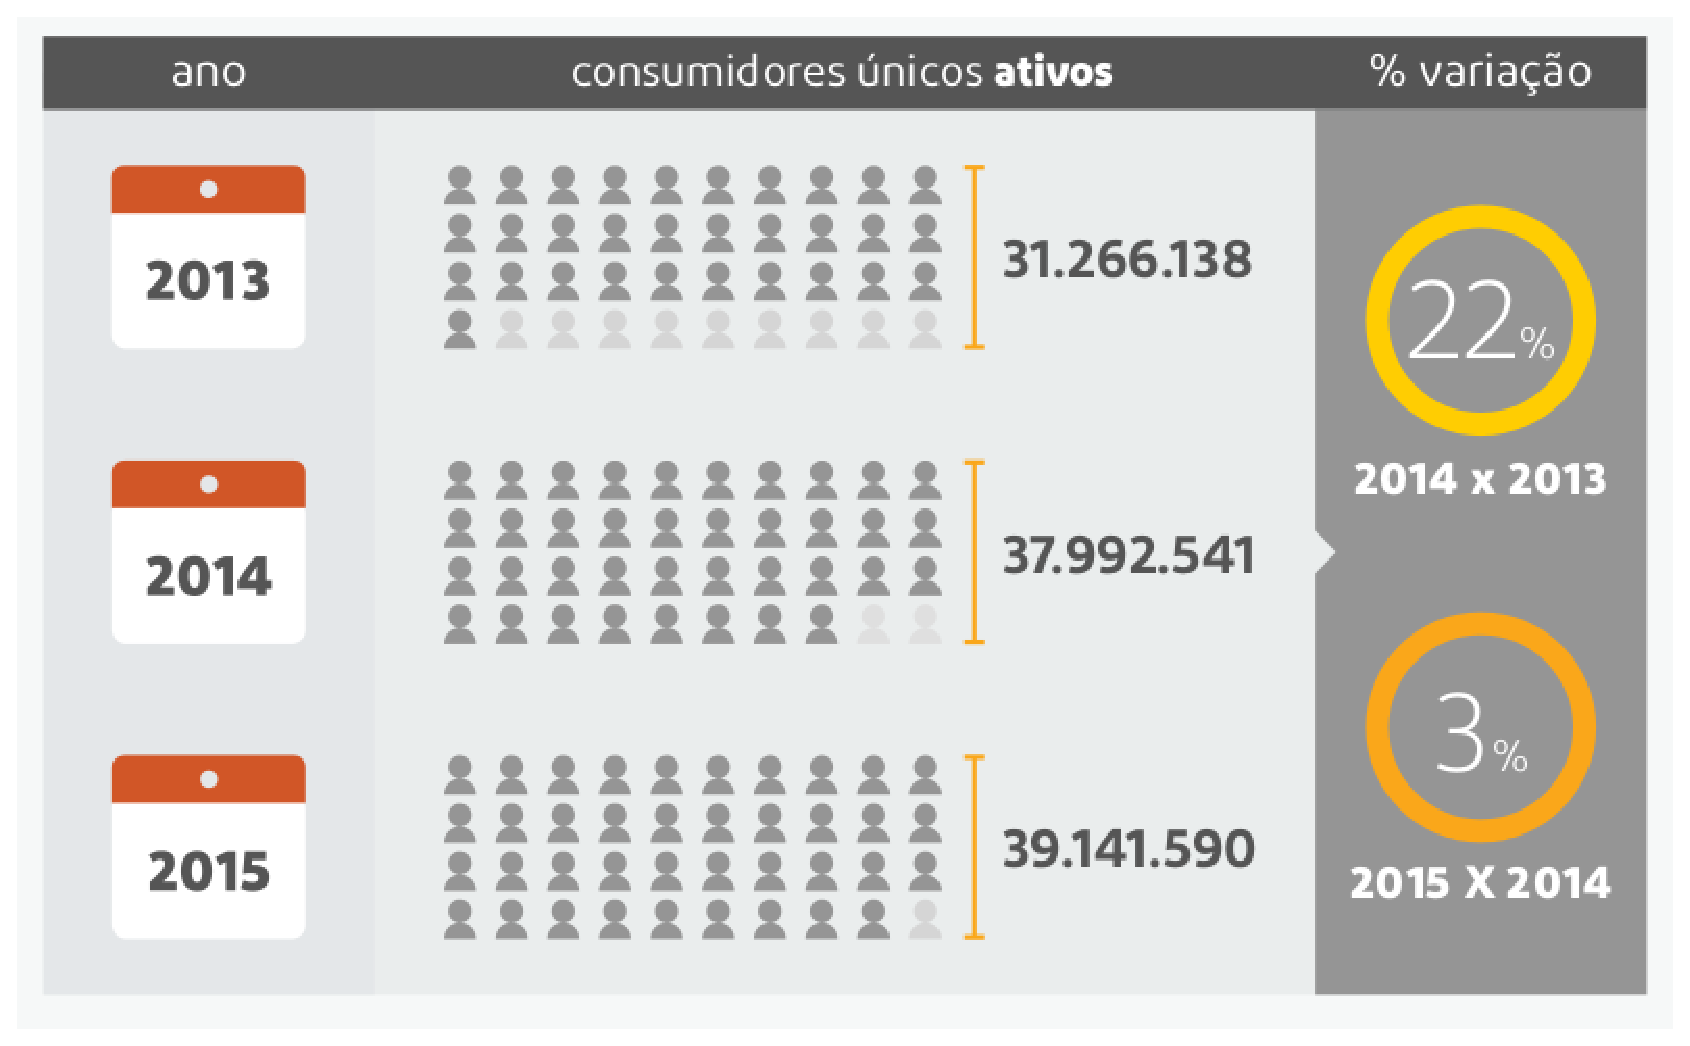
\includegraphics[width=12cm]{img/webshoppers/consumidores.eps}
\caption{Consumidores únicos ativos}
\small{Fonte: E-Bit/Buscapé - Relatório WebShoppers}
\label{figura:consumidores}
\end{figure}

Na figura \ref{figura:consumidores} podemos notar que a quantidade de e-consumidores ativos (pessoas que efetivaram pelo
menos uma compra virtual, ao longo de 2015) apresentou pequeno crescimento, se comparada com anos anteriores. Em 2015, esse número chegou ao total de 39,1 milhões de consumidores. O número de pedidos e o faturamento do comércio eletrônico também foram notavalmente altos. Com um total de 106,2 milhões em 2015, o incremento no número de pedidos no mercado brasileiro foi de 3\%,
em relação a 2014. Ver figura \ref{figura:pedidos}. O faturamento do comércio eletrônico foi de R\$ 41,3 bilhões. O número representa um crescimento nominal de 15,3\%, em relação a 2014, quando as vendas somaram um total de R\$ 35,8 bilhões como pode ser visto na figura \ref{figura:vendas}.

\begin{figure}[H]
\centering
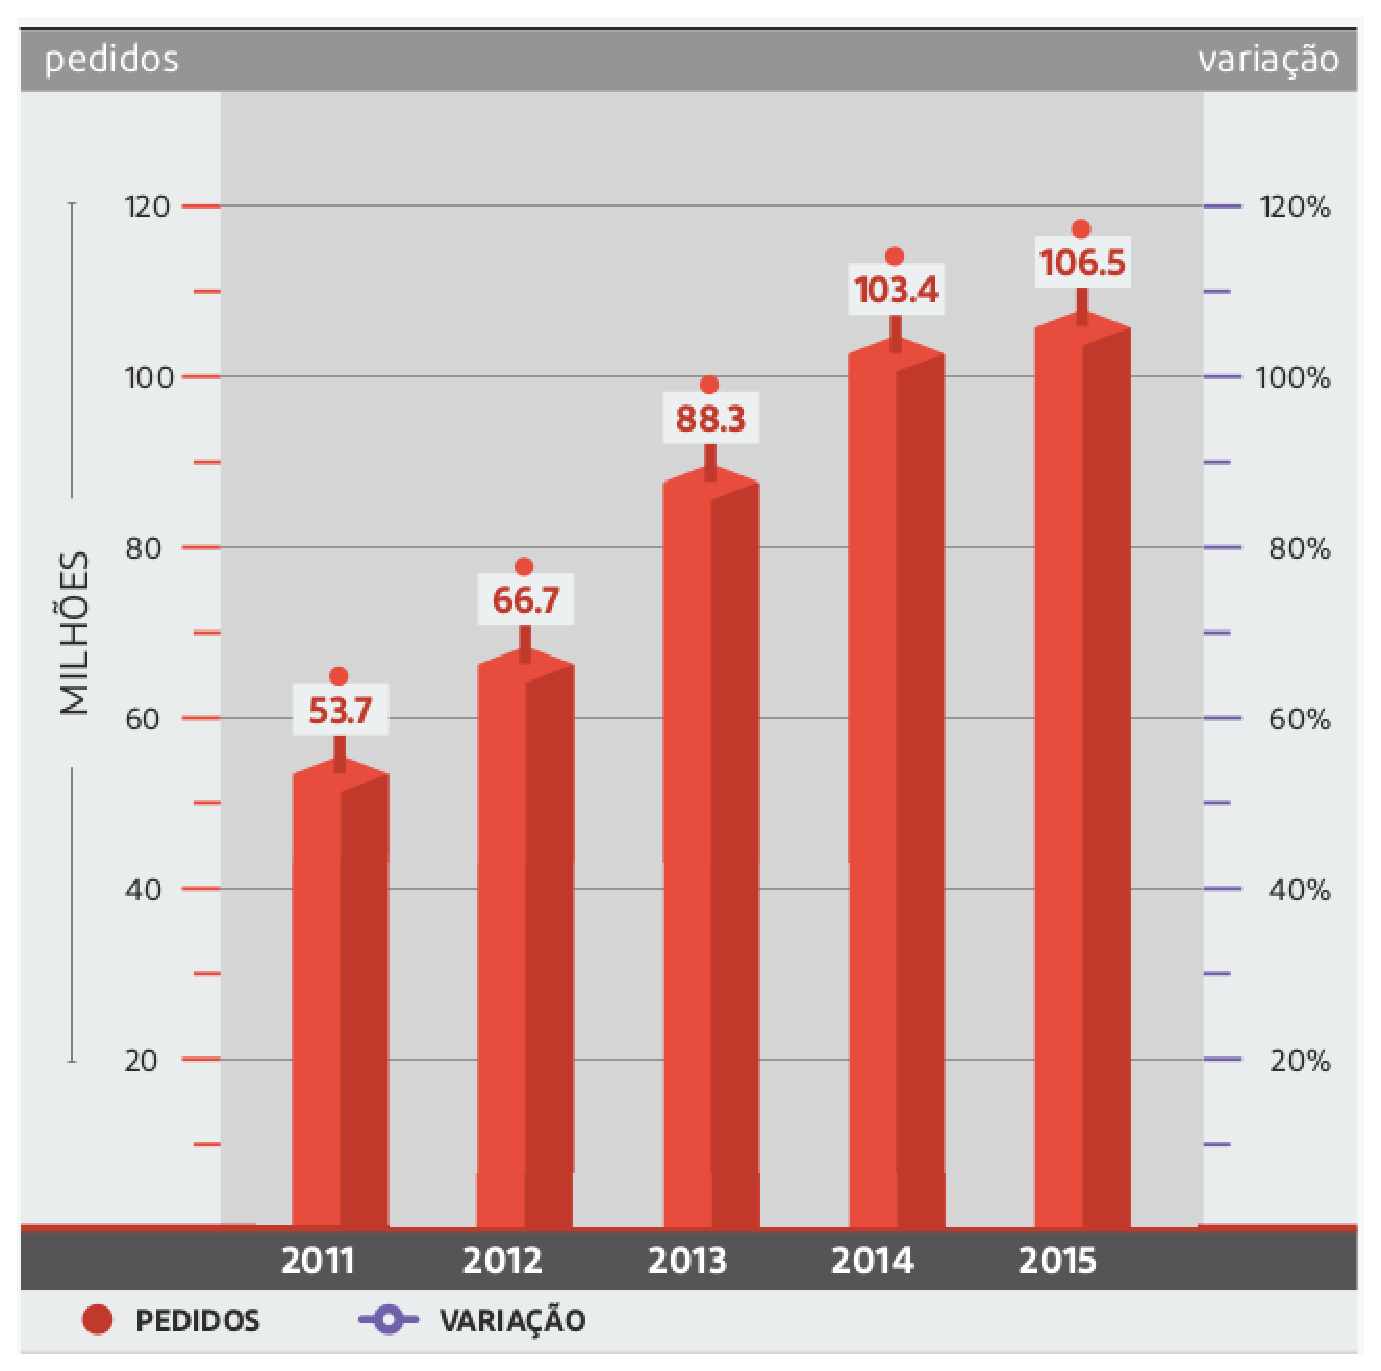
\includegraphics[width=10cm]{img/webshoppers/total-pedidos.eps}
\caption{Total de pedidos realizados no \textit{e-commerce} no Brasil}
\small{Fonte: E-Bit/Buscapé - Relatório WebShoppers}
\label{figura:pedidos}
\end{figure}

\begin{figure}[H]
\centering
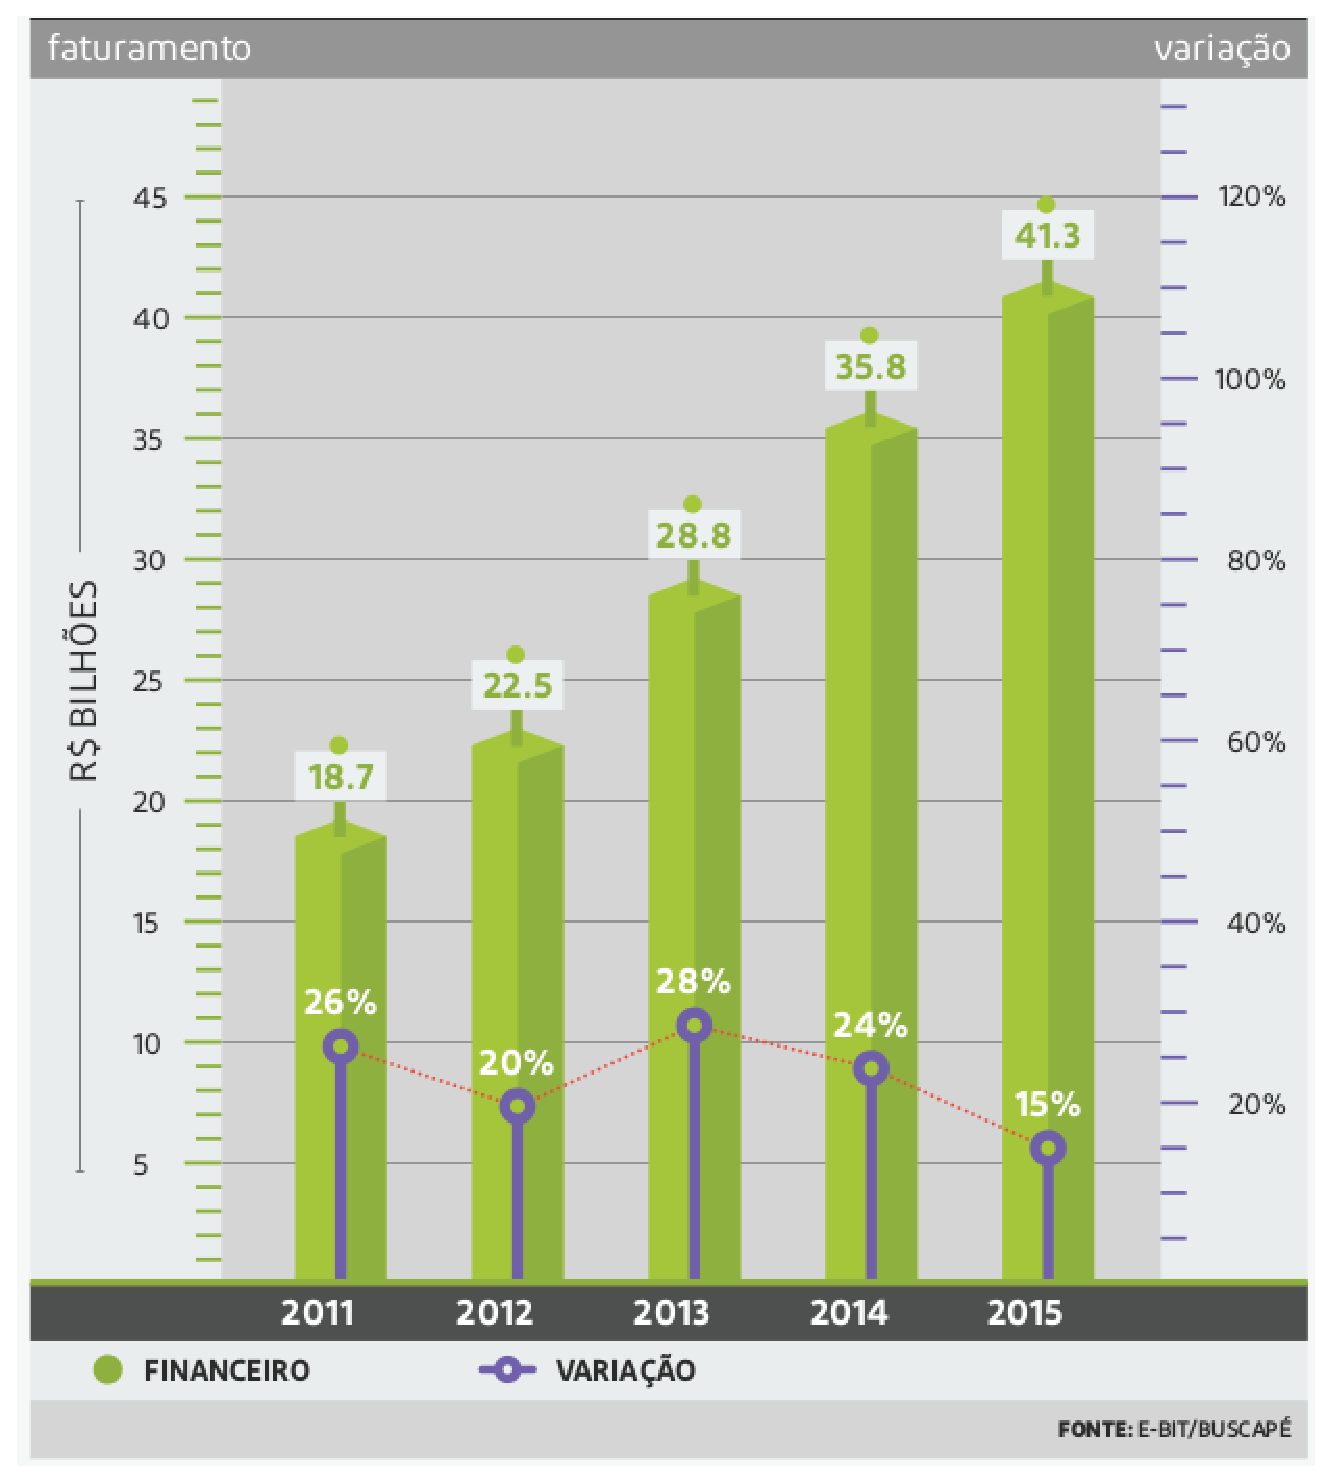
\includegraphics[width=10cm]{img/webshoppers/faturamento.eps}
\caption{Total de faturamento do \textit{e-commerce} no Brasil}
\small{Fonte: E-Bit/Buscapé - Relatório WebShoppers}
\label{figura:vendas}
\end{figure}

O relatório também destaca dados sobre a satisfação dos clientes em realizar suas compras na internet. O Net Promoter Score (NPS) é um indicador que mensura a satisfação e a fidelização dos clientes. No balanço geral do ano, o NPS apresentou o melhor resultado. Ver figura \ref{figura:nps}.

\begin{figure}[H]
\centering
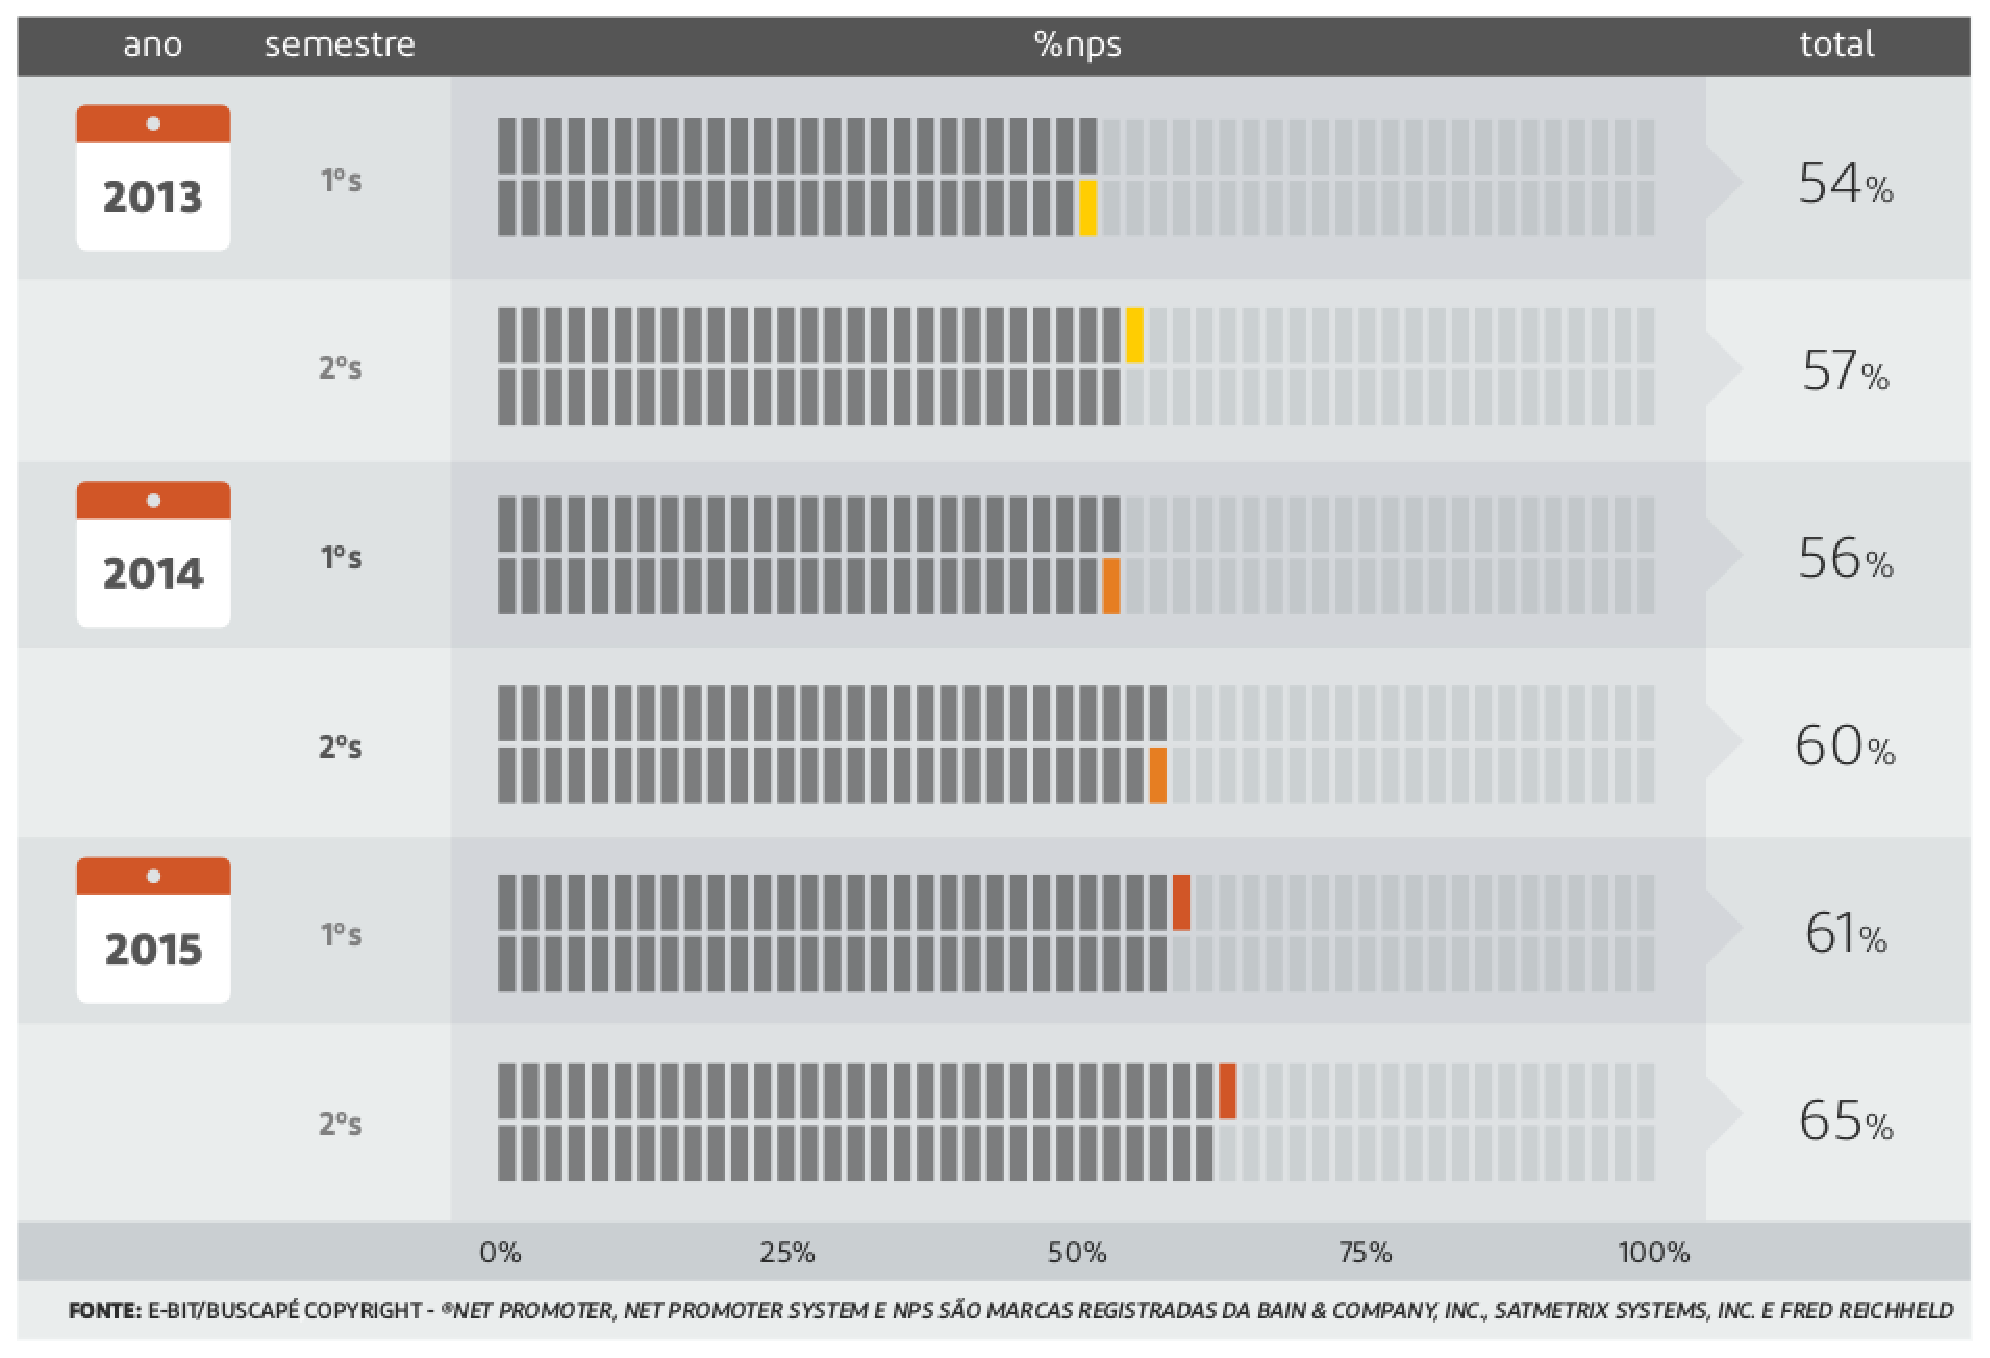
\includegraphics[width=12cm]{img/webshoppers/nps.eps}
\caption{Satisfação e fidelização de clientes}
\small{Fonte: E-Bit/Buscapé - Relatório WebShoppers}
\label{figura:nps}
\end{figure}

Vitor Augusto Meira França, economista da Fecomercio-SP principal entidade sindical paulista dos setores de comércio e serviços. Responsável por administrar, no Estado, o Serviço Social do Comércio (Sesc) e o Serviço Nacional de Aprendizagem Comercial (Senac) afirma o seguinte:

\begin{citacao}
Diante de um quadro de instabilidade política, inflação alta, taxas de juros elevadas, escassez de crédito, aumento do desemprego e consequente conservadorismo dos consumidores, o varejo brasileiro deve repetir o fraco desempenho do ano passado e registrar nova queda das vendas neste ano. por outrolado, o e-commerce deve apresentar crescimento como ocorreu em 2015. \cite{webshoppers}
\end{citacao}

O Relatório \textit{WebShoppers} apresenta estimativas sobre esse crescimento, que podemos ver nas figuras \ref{figura:estimativa:pedidos} e \ref{figura:estimativa:faturamento}.

\begin{figure}[H]
\centering
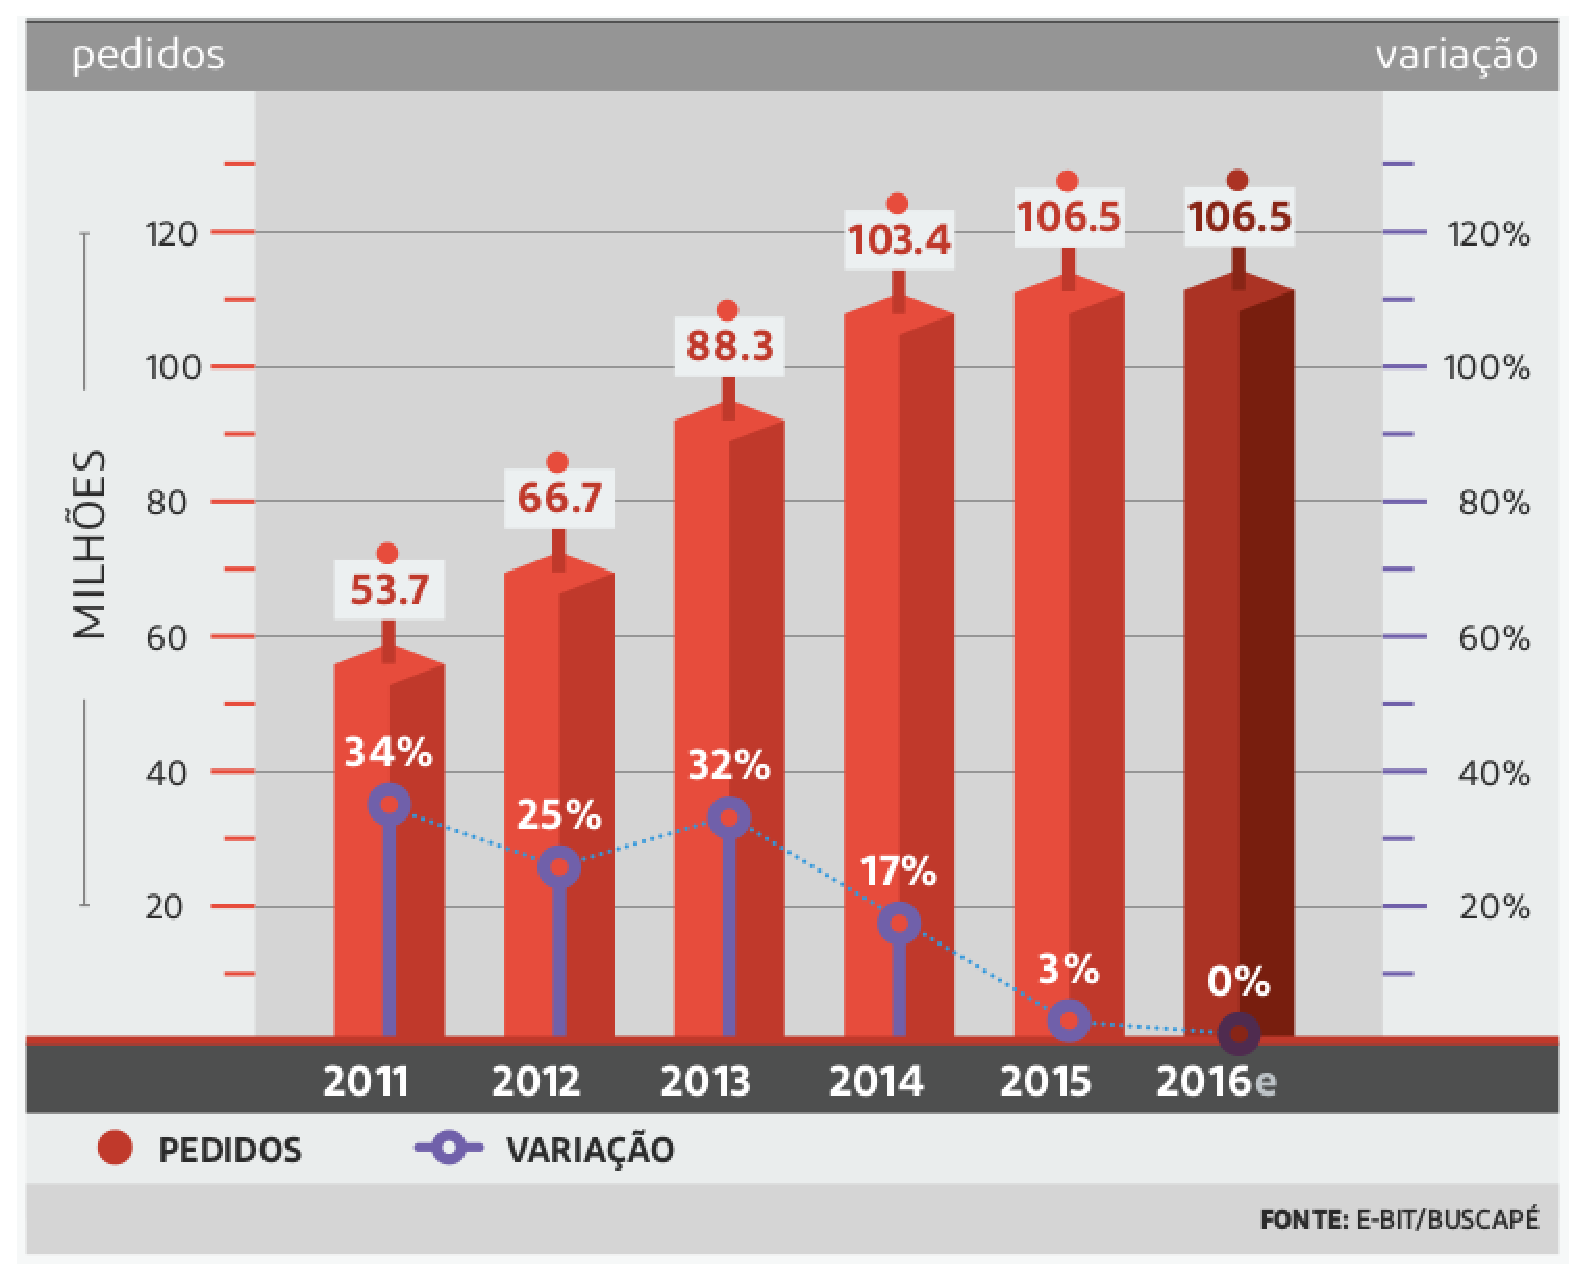
\includegraphics[width=12cm]{img/webshoppers/estimativa-pedidos.eps}
\caption{Estimativa do número de pedidos no \textit{e-commerce} para 2016}
\small{Fonte: E-Bit/Buscapé - Relatório WebShoppers}
\label{figura:estimativa:pedidos}
\end{figure}

\begin{figure}[H]
\centering
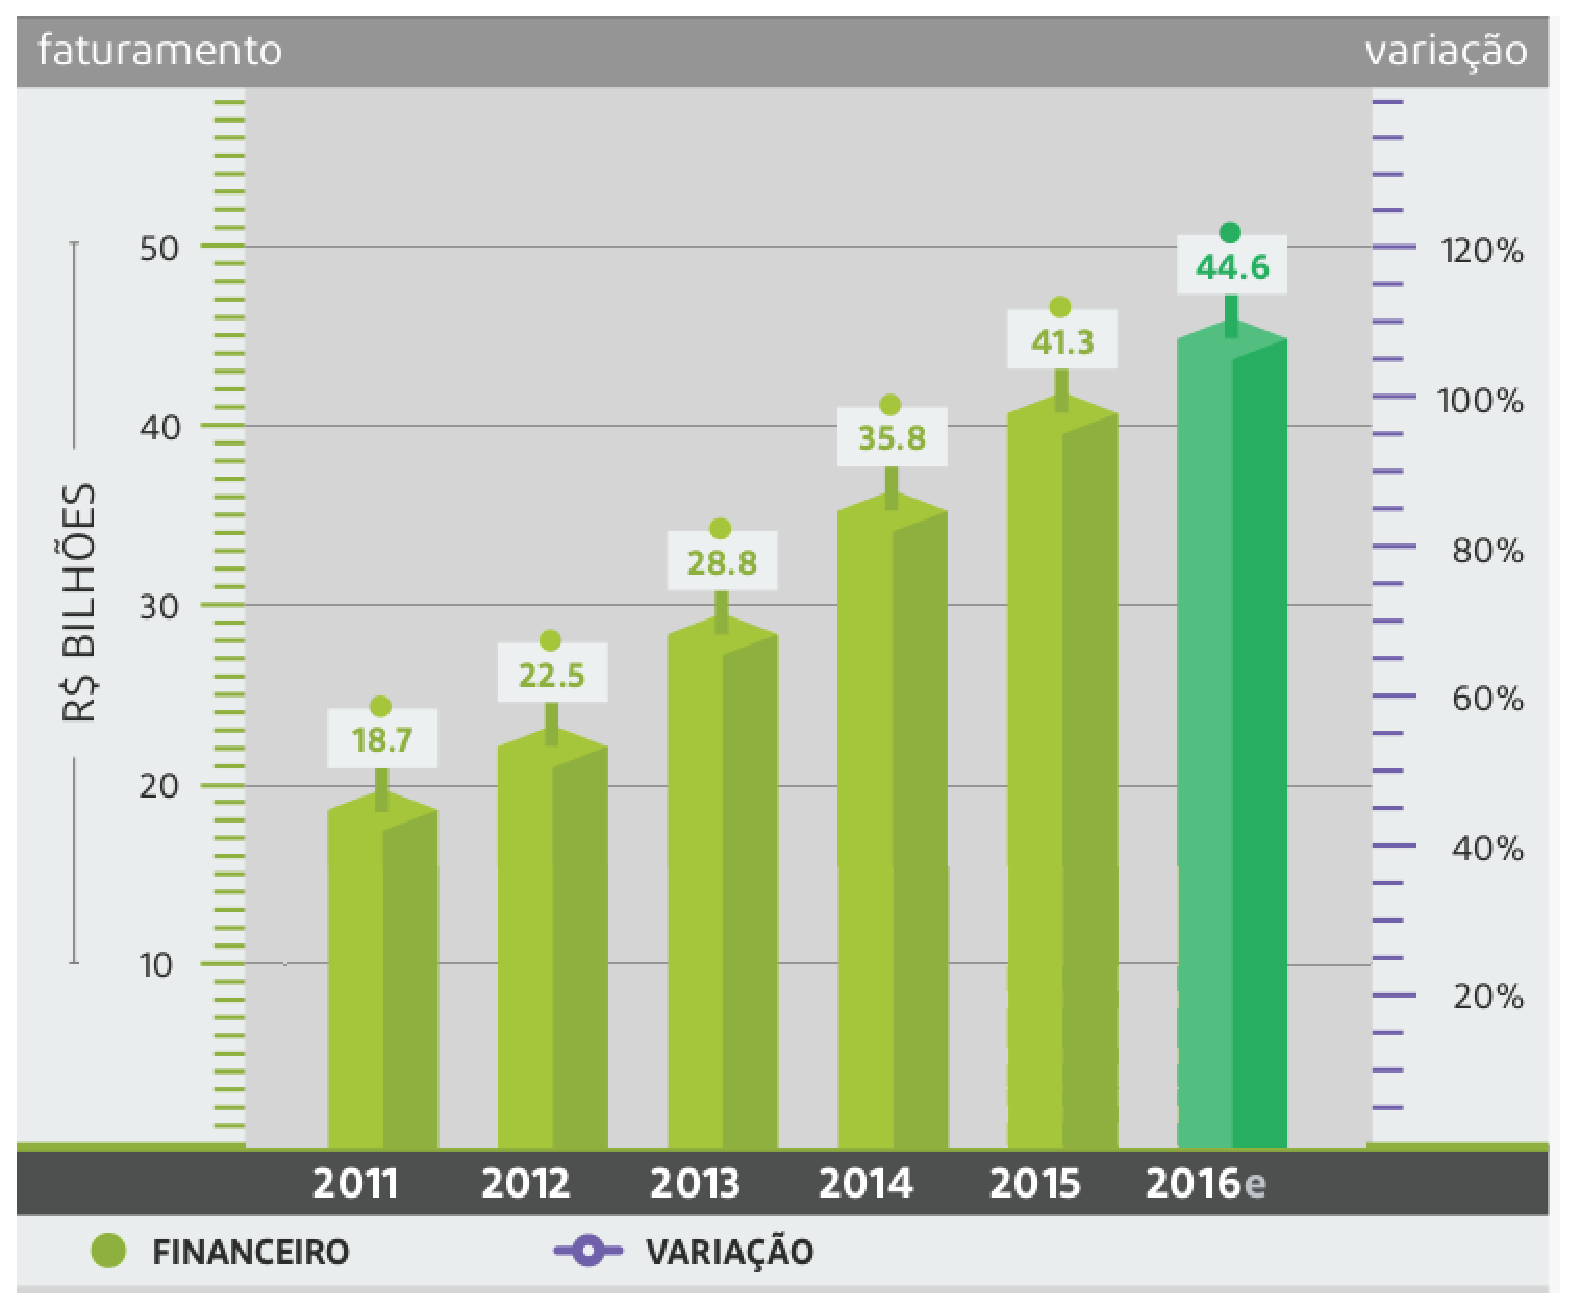
\includegraphics[width=12cm]{img/webshoppers/estimativa-faturamento.eps}
\caption{Estimativa de faturamento do \textit{e-commerce} para 2016}
\small{Fonte: E-Bit/Buscapé - Relatório WebShoppers}
\label{figura:estimativa:faturamento}
\end{figure}

Após essa breve análise da situação do \textit{e-commerce} no brasil, podemos afirmar que o comércio eletrônico é sem dúvidas um excelente negócio. 

Entre os empresários que se aventuram nesse ambiente, um dos anseios é ter uma loja que tenha a identidade visual da sua marca, que possibilite formas práticas e seguras de compra pelos clientes e, claro, que seja de fácil manuseio e administração para ele mesmo. Com ferramentas como o Mercado Livre\footnote{https//www.mercadolivre.com.br}, por exemplo, é possível disponibilizar produtos para a venda, mas em um ambiente diferente de uma loja virtual particular.
% chapter introdução(end)

\section{Motivação} % (fold)
\label{sec:motivacao}

Existem muitas ferramentas que facilitam a criação e gestão de lojas virtuais, porém não são populares e as vezes desconhecidas, tais ferramentas poderiam ajudar a expandir um negócio ou criar uma oportunidade para aqueles que desejam empreeder através de vendas na Internet. 

Segundo \citeonline{felipini}, ``Um e-commerce pode ser implantado aos poucos e testado''. Diferentemente de uma empresa tradicional, em que o início das operações ocorre somente com o empreendimento totalmente estruturado, um negócio na Internet pode ser implantado em etapas, o que dilui o investimento e facilita a correção de erros. Por exemplo, um estabelecimento de vendas só receberá seu primeiro cliente após a loja estiver totalmente pronta. Na Internet, você pode montar um site de conteúdo, com ou sem sua marca definitiva, testar a aceitabilidade de seu modelo de negócio e produtos, avaliar a visitação e, somente depois, começar a vender. Dessa forma, mesmo aqueles que ainda não possuam um negócio, poderão investir em um \textit{e-commerce}.

Os comerciantes já fixados no mercado e interessados em colocar seu negócio na rede, procuram por empresas especializadas em desenvolvimento de softwares para desenvolver seu site de vendas. O problema nisso é que o custo pode ser alto. \citeonline{jalote} afirma: ``O software é caro porque torna se uma atividade difícil e trabalhosa de ser realizado pelo engenheiro de software''.  Outro problema realacionado ao desenvolvimento de software no geral, isso inclúi uma loja virtual, é o tempo. O que gera insatisfação dos clientes, pela demora no cumprimento dos prazos \cite{pressman}.

Além desses, um outro problema é a manutenção do site. Segundo \citeonline{sommervile} manutenção de software é a modificação de um programa após ter sido colocado em uso. Mundanças por exemplo, em alterar o layout\footnote{Estrutura visual das páginas/janelas do sistema} geram custos e podem também ser demoradas.

A Sudo Loja, visa resolver esses problemas oferecendo um CMS (do inglês \textit{Content Management System}), capaz de criar, gerenciar e tornar possível a personalização de uma loja virtual. O CMS proposto busca facilitar a criação e gestão de um \textit{e-commerce}, promovendo uma entrada rápida ao mercado virtual à pequenas e médias empresas. Podem ser vistos vários sistemas que funcionam dessa maneira, como por exemplo: a \citeonline{tray} e \citeonline{lojaintegrada}. Na Seção \ref{cha:ferramentas_relacionadas} será apresentado um comparativo entre estas e outras ferramentas.


% section motivacao (end)

\section{Objetivos} % (fold)
\label{sec:objetivos}

Esta seção apresenta os objetivos que direcionarão a construção do sistema.

\subsection{Objetivo Geral} % (fold)
\label{sub:objetivo_geral}

Esse trabalho tem como objetivo principal o desenvolvimento de uma ferramenta para criação de lojas virtuais, onde um usuário cadastrado poderá criar um ou mais lojas, personalizar seu \textit{layout} e disponibilizar produtos para a venda.

% subsection objetivo_geral (end)

\subsection{Objetivos Específicos} % (fold)
\label{sub:objetivos_espec}

\begin{itemize}
\item Prover uma alternativa de \textit{e-commerce} para a região.
\item Tornar acessível financeiramente, manter seu próprio \textit{e-commerce}.
\item Incentivar o uso de novas soluções em TI nas pequenas e médias empresas comerciais da região.
\item Facilitar a entrada de novos comerciantes no mercado virtual
\end{itemize}
% subsection objetivos_espec (end)

% section objetivos (end)

\section{Organização do Documento} % (fold)
\label{sec:organizacao_do_documento}

% section organizacao_do_documento (end)
A Seção \ref{cha:fundamentaco_teorica} apresenta a fundamentação teórica para o desenvolvimento deste trabalho. Na Seção \ref{cha:metodologia} é descrita a metodologia adotada para execução do projeto. A seção \ref{cha:metodologia} descreve os métodos e o tipo de pesquisa realizada no trabalho . A Seção \ref{cha:sudoloja} descreve a análise, o projeto, a implementação e a validação do sistema. A Seção \ref{cha:consideracoes_finais} apresenta as considerações finais do trabalho. E por fim, o apêndice.

\chapter{Fundamentação Teórica} % (fold)
\label{cha:fundamentaco_teorica}

\section{CMS} % (fold)
\label{sec:cms}

Sistemas de Gerenciamento de Conteúdo (SGC) ou Content Management System (CMS), segundo \citeonline{mercer} são softwares que facilitam a criação, organização, manipulação e remoção de dados em forma de imagens, documentos, scripts, textos, etc.
Já \citeonline{barcia}, diz que um CMS, é uma plataforma de gestão de conteúdos, ou seja, um sistema que integra ferramentas que permitem criar, editar e publicar conteúdo em tempo real, onde os utilizadores manipulam uma interface sem terem a necessidade de saber programar. \citeonline{barcia} ainda ressalta que os gerenciadores também dispensam o uso de programação, facilitando dessa forma a gestão dos dados e o acesso às funcionalidades da ferramenta.

O uso de um CMS pode facilitar o trabalho dos administradores de aplicações, que envolvem muitas atualizações no seu conteúdo, como por exemplo, blogs, portais corporativos\footnote{Instrumento de gestão de informação e de conhecimento}. ``Os benefícios ligados a adoção de um CMS incluem desde a redução do custo de atualização dos conteúdos nos websites até o aumento da eficiência das equipes de TI'' \cite{pereira}.

Em linhas gerais, um CMS permitiria administrar conteúdos em meio digital. E para o caso particular que nos ocupa, um CMS permitiria gerenciar os conteúdos de uma loja virtual.

Em outras palavras, um CMS é uma ferramenta que permite a um editor criar e publicar qualquer tipo de informação em uma página web. Geralmente, um CMS trabalha manipulando um banco de dados, de modo que o editor simplesmente atualiza este banco, incluindo nova informação ou editando a existente.

Contudo, o mais interessante, é que essa ferramenta é feita de tal maneira que mesmo aqueles que nunca ouviram falar de JAVA, PHP, MySQL, Javascript ou qualquer outra linguagem voltada para web poderá usá-lo, inclusive esta é sua principal função, tornar acessível a todos a sua presença na Internet através de um site, facilitando a inserção de textos, de comentários e dezenas de outras funcionalidades, de acordo com as características de cada aplicação. Alguns Exemplos de CMS podem ser vistos a seguir.

\begin{itemize}
\item \textit{Drupal} - É uma plataforma de gerenciamento de conteúdo de código aberto, usado em milhares de web sites e aplicações. Ele é desenvoldivo, usado, e apoiado por uma comunidade ativa e diversificada de pessoas ao redor do mundo \cite{drupal}.

\item \textit{OpenText} \citeyear{opentext} - O primeiro sistema CMS comercial que apareceu no mercado. A OpenText é líder em Gestão de Informação Corporativa. Seus produtos de gerenciamento de conteúdo permitem uma coleta mais eficiente de todos os tipos de informação - estruturada e não estruturada - e fornecem essa informação em contexto por qualquer aplicativo, plataforma ou processo \cite{opentext}.

\item \textit{Wordpress} - Sistema muito popular e bastante usado pelos \textit{bloggers}. WordPress é um software web que você pode usar para criar um site, blog, ou app \cite{wordpress}.
\end{itemize}

% section cms (end)

\section{\textit{E-commerce}} % (fold)
\label{sec:e_commerce} 

Segundo \citeonline{kalakota}, o Comércio Eletrônico (CE) pode ser definido como sendo a compra e a venda de informações, produtos e serviços através de redes de computadores. \citeonline{bloch} estenderam esta definição incluindo que CE é o suporte para qualquer tipo de transações de negócio sobre uma infra-estrutura digital.

\apudonline{kalakota}{albertin} há muito tempo, consideravam que o ambiente tradicional de negócio estava mudando rapidamente, com os consumidores e negócios procurando flexibilidade para mudar os parceiros de negócio, plataformas, carreiras e redes. O \textit{e-commerce} começava a se disseminar.

O comércio eletrônico ou \textit{e-commerce}, é aplicável a qualquer tipo de transação comercial que pode envolver compra, venda, transferência ou troca de produtos, serviços ou informações por meio de redes de computadores, incluindo a Internet \cite{turban}.

Existem diferenças entre \textit{e-commerce} e \textit{e-business}. \textit{E-business} é definido como o uso das tecnologias da informação para executar funções de negócios. \textit{E-business} é, portanto, um termo mais amplo que inclui \textit{e-commerce} \cite{gordon}. 

Dentre os modelos existentes de \textit{e-business}, \citeonline{asfoura} destaca três tipos principais que incluem o e-commerce em sua execução:

\begin{itemize}
\item \textbf{Empresa para Empresa (B2B – Business to Business):} Engloba as negociações de bens ou serviços que acontecem entre empresas;
\item \textbf{Empresa para Consumidor (B2C – Business to Consumer):} Tipo de comércio mais conhecido, onde a empresa faz o negócio diretamente com os consumidores finais;
\item \textbf{Consumidor para Consumidor (C2C – Consumer to Consumer):} Engloba todas as transações que acontecem entre consumidores finais, geralmente intermediadas por uma terceira entidade;
\end{itemize}

O sistema que será apresentado se encaixa no modelo de negócio B2C (\textit{Business to Consumer}), onde o lojista fará o negócio diretamente com os consumidores finais.


% section e_commerce (end)
% chapter fundamenta_o_te_rica (end)

\bibliography{referencias}

% Inicio do Apêndice
% \appendix
% \newpage
% \phantomsection
% \addcontentsline{toc}{chapter}{Apêndice}  
% \addtocontents{toc}{\protect\setcounter{tocdepth}{-1}}
% \chapter{Documento de Visão}
% \label{ap:documento_visao}
% \section{Introdução} % (fold)
% \label{sec:Introducao}

% Este documento apresenta uma solução de software para ser apresentado como TCC 1, solicitado pelos professores. Como cliente Francisco Paulo de Freitas Neto (Orientador). Apresenta também os problemas a serem solucionados, as necessidades dos principais envolvidos, o alcance do projeto e as funcionalidades esperadas do sistema.

% \subsection{Objetivos} % (fold)
% \label{sec:objetivos}

% Como objetivo principal, esse projeto visa facilitar o ingresso de um comerciante ao mercado virtual, fornecendo uma ferramenta capaz de criar uma loja virtual onde um usuário, sem ajuda especializada, poderá gerenciar e customizar sua loja de maneira simples e intuitiva.

% % subsection objetivos (end)

% \subsection{Abrangência do Projeto} % (fold)
% \label{sec:abrengencia_do_projeto}

% Esse projeto é voltado ao âmbito comercial, contemplando todos aqueles que desejam criar uma loja virtal e disponibilizar produtos à venda. A loja terá integração com o serviço Google Shopping permitindo que compradores encontrem  informações do produto no Google de forma rápida e fácil.
% O produto final será uma plataforma onde qualquer usuário cadastrado poderá criar, gerenciar e personalizar uma loja virtual.


% % subsection abrengencia_do_projeto (end)

% \subsection{Definições, Acrônimos e Abreviações} % (fold)
% \label{sec:siglas}

% \textbf{CMS} – Content Management System (Sistema de Gerenciamento de Conteúdo)

% % subsection siglas (end)
% \subsection{Organização do Documento} % (fold)
% \label{sec:organizacao_do_documento}

% As próximas seções trataram sobre a descrição do problema, as partes envolvidas e tipos de usuários que utilizaram o sistema, a solução proposta para os problemas elencados, logo após, as funcionalidades oferecidas por esta solução, seguidas pelas restrições do sistema. Também poderão ser vistos alguns protótipos na Seção \ref{sec:prototipos}.

% % subsection organizacao_do_documento (end)
% % section Introdução (end)

% \section{Descrição do Problema} % (fold)
% \label{cha:descricao_do_problema}

% \begin{itemize}
% \item Dificuldades no gerenciamento de uma loja virtual - 
% Aqueles que desejam entrar no mercado virtual geralmente recorrem a empresas de desenvolvimento de software para criar sua loja virtual, e geralmente, qualquer tipo de modificação a ser feita, seja no conteúdo ou no \textit{layout} e estilo do site, necessita da intervenção direta da equipe de desenvolvimento.

% \item Afeta - O lojista.
% \item O impacto deste problema é - 
% Um grande impacto que isso causa para o lojista é a demora, tanto no desenvolvimento quanto na modificação de alguma parte da loja online, por exemplo, digamos que por algum motivo o lojista queira modificar o estilo do sua loja online. A equipe então, levará um certo tempo (dependendo da complexidade de modificação) até entender completamente o que o cliente deseja para então realizar a modificação e deixar a loja do jeito que o cliente pediu, e é claro, na maioria dos casos com um custo considerável. Então temos dois problemas principais: demora e custo.

% \item Uma solução ideal permitiria - 
% Fornecer um sistema que possibilitasse a criação, personalização  e gerenciamento de uma loja online sem intervenção de pessoal especializado, com um baixo custo.

% \end{itemize}

% % section descricao_do_problema (end)

% \section{Partes Envolvidas} % (fold)
% \label{sec:partes_envolvidas}

% Os principais envolvidos serão descritos nas seções \ref{sec:resumo_dos_envolvidos} e \ref{sec:resumo_dos_usuarios}.

% \subsection{Resumo dos Envolvidos} % (fold)
% \label{sec:resumo_dos_envolvidos}

% Os envolvidos que se interessam em empenhar-se nesse projeto, são os desenvolvedores, os comerciantes, e os consumidores.

% % subsection resumo_dos_envolvidos (end)

% \subsection{Resumo dos Usuários} % (fold)
% \label{sec:resumo_dos_usuarios}

% Uma lista resumida de todos os usuários identificados pode ser vista no Quadro \ref{quadro:usuarios}.

% \begin{table}[H]
% \centering
% \begin{tabular*}{\textwidth}{@{\extracolsep{\fill}} |p{3cm}|p{4cm}|p{4cm}|p{3cm}|}
% \hline
% \rowcolor{ballblue}
% Nome & 	Descrição & Responsabilidades & Envolvido \\

% Lojista & 
% Administrador da loja virtual & 
% Criação da loja, Personalização da loja, Inclusão de dados no sistema, Gerenciamento de pedidos 
% & Dono do negócio ou alguém que represente seus interesses	

% \\
% \hline

% Cliente &
% Consumidor dos produtos oferecidos na loja &
% Efetuar cadastro para realização de uma compra &
% Qualquer consumidor em potencial que deseje  realizar uma compra  (de um ou mais)  produtos oferecidos pela loja

% \\	
% \hline

% \end{tabular}
% \caption{Resumo dos usuários}
% \label{quadro:usuarios}
% \end{table}

% % subsection resumo_dos_usuarios (end)

% % section partes_envolvidas (end)

% \section{Descrição da Solução Proposta} % (fold)
% \label{sec:descri_o_da_solu_o_proposta}

% A solução proposta é um sistema computacional web para criação de lojas virtuais (um CMS voltado para criação de lojas, onde um usuário poderá criar, personalizar as suas lojas virtuais e assim, disponibilizar os seus produtos para venda) e uma área para perguntas ao vendedor sobre um produto desejado. tudo isso de forma simples sem conhecimento especializado, sem burocracias. 

% % section descri_o_da_solu_o_proposta (end)

% \section{Funcionalidades} % (fold)
% \label{sec:funcionalidades}

% No Quadro \ref{quadro:funcionalidades} podemos ver uma breve descrição das funcionalidades do produto, com um nível de detalhamento genérico para uma melhor compreensão.


% \begin{longtable}{|p{7cm}|p{7cm}|}
% \hline
% \rowcolor{ballblue}
% Funcionalidade & Descrição	\\	
% Gerenciamento de produtos & Inclusão, remoção e alteração de produtos, cadastro de múltiplas imagens para cada produto
% \\	
% \hline
% Gerenciamento de pedidos & Controle de todos os pedidos realizados
% \\	
% \hline
% Personalização da loja & A loja poderá ser personalizada totalmente (\textit{layout}, cores, fontes, edição de CSS e HTML)
% \\	
% \hline
% Gerenciamento de clientes & Cadastro, alteração de dados cadastrais, remoção da conta.
% \\	
% \hline
% Calculo de frete automático quando houver & Caso haja frete sobre um produto da loja, em tempo real o cliente poderá ver o valor do frete
% \\	
% \hline
% Divulgação & Resultados de pesquisas sobre produtos cadastrados na loja poderão aparecer facilmente nas buscas do google através do Google Shopping, aumentando as chances do produto ser encontrado.
% \\	
% \hline
% Controle de estoque & O estoque poderá ser consultado e gerenciado, contendo opções como desabilitar/habilitar produtos, visualizar quantidade de cada produto, filtrar produtos por nome
% \\	
% \hline
% Acompanhamento de pedidos para os clientes & Os clientes poderão visualizar o status do pedido a qualquer momento,
% \\	
% \hline
% \caption{Resumo das Funcionalidades}
% \label{quadro:funcionalidades}
% \end{longtable}	


% % section funcionalidades (end)

% \section{Restrições do Projeto} % (fold)
% \label{sec:restricoes_do_projeto}

% O sistema será uma aplicação WEB com design totalmente responsivo, o que significa que poderá ser utilizado tanto pelo navegador de um computador desktop, quanto pelo navegador do celular. Não possuirá restrições quanto ao sistema operacional utilizado pelo consumidor.

% % section restricoes_do_projeto (end)

% \section{Protótipos} % (fold)
% \label{sec:prototipos}

% \begin{figure}[H]
% \centering
% 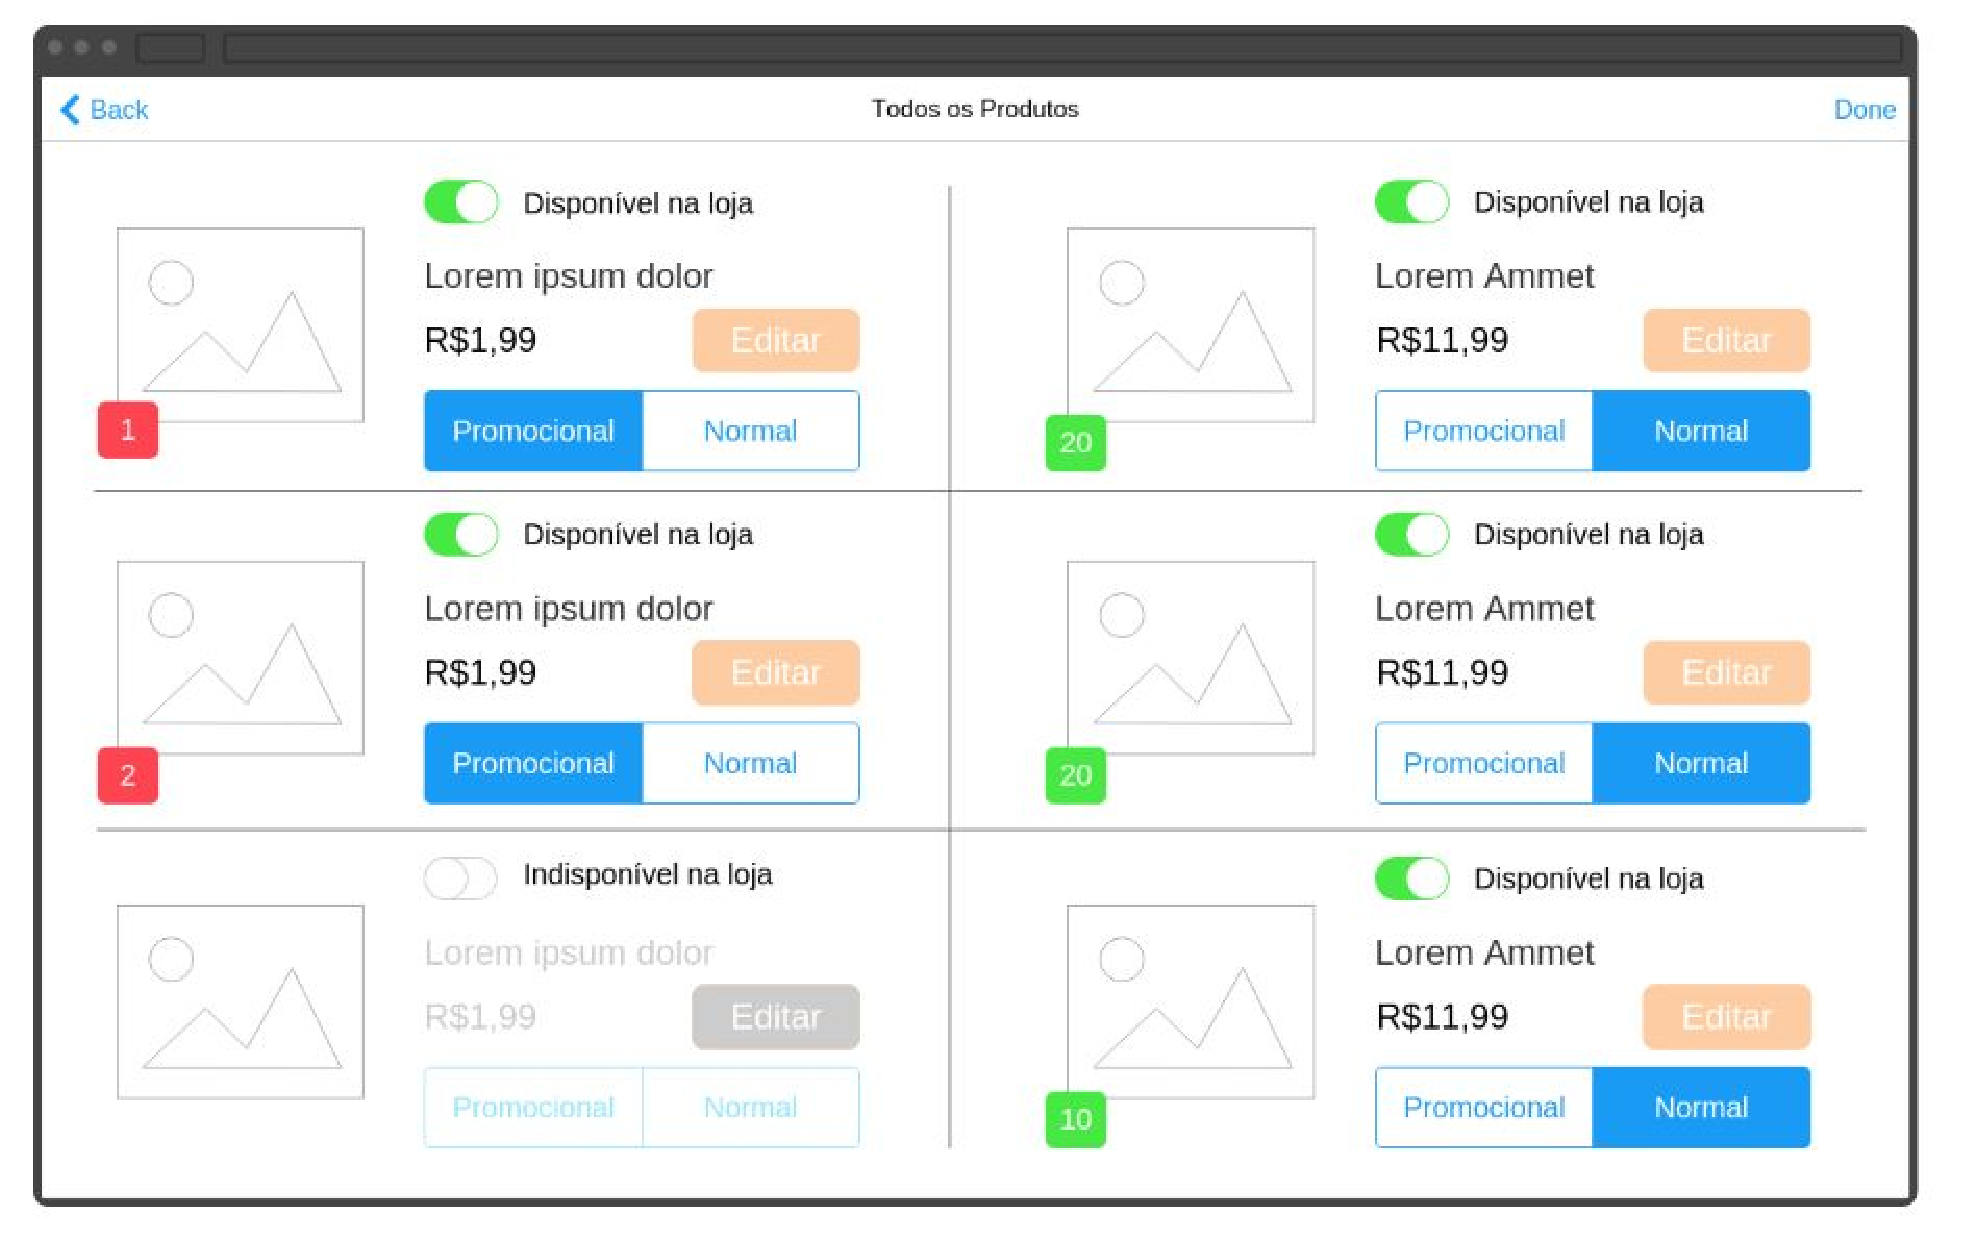
\includegraphics[width=12cm]{img/prototipos/produtos-cadastrados.eps}
% \caption{Visualização de produtos cadastrados}
% \label{figura:produtos_cadastrados}
% \end{figure}

% \begin{figure}[H]
% \centering
% 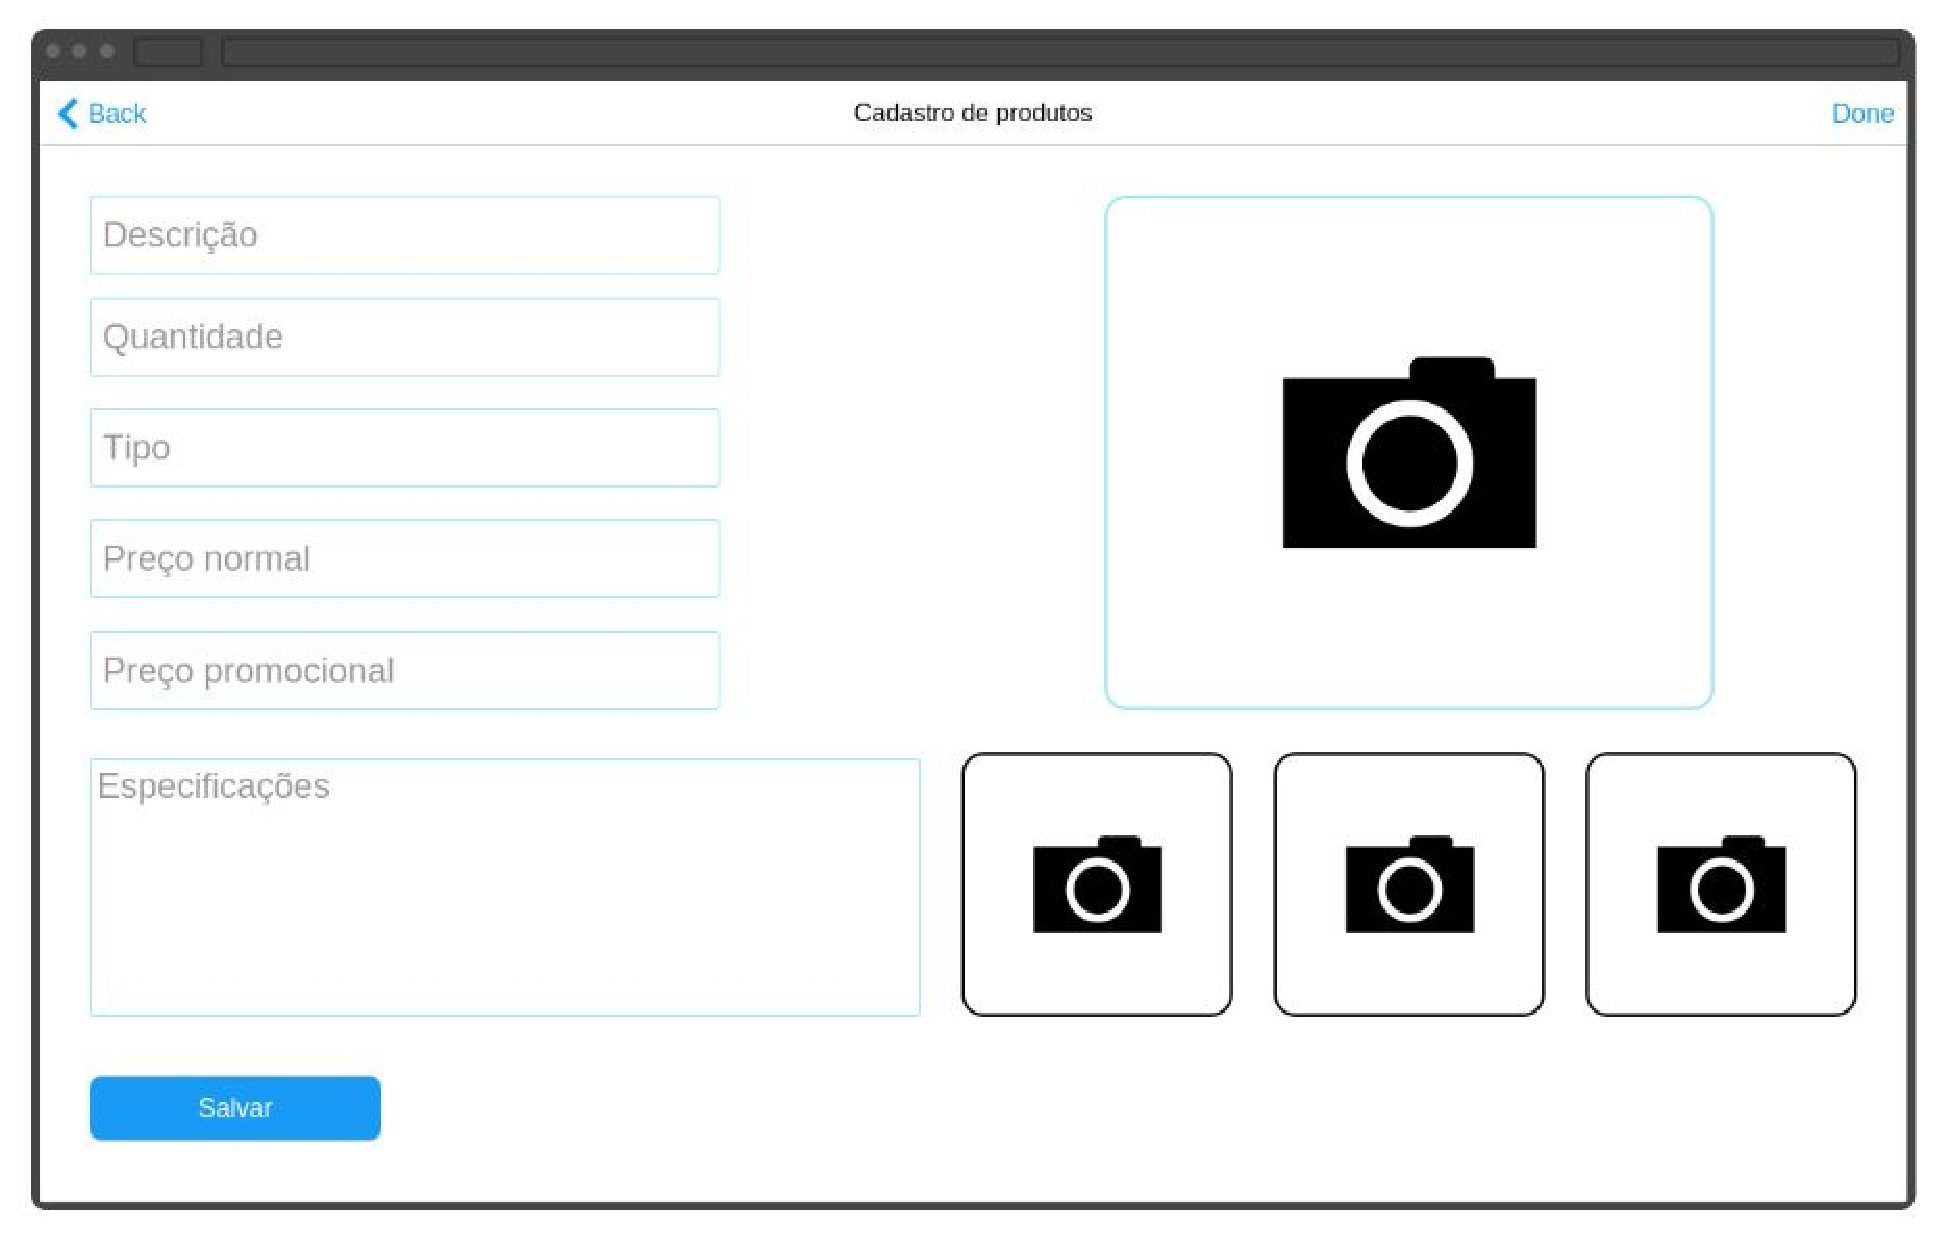
\includegraphics[width=12cm]{img/prototipos/cadastro-produto.eps}
% \caption{Cadastro de produtos}
% \label{figura:Cadastro_de_Produtos}
% \end{figure}

% \begin{figure}[H]
% \centering
% 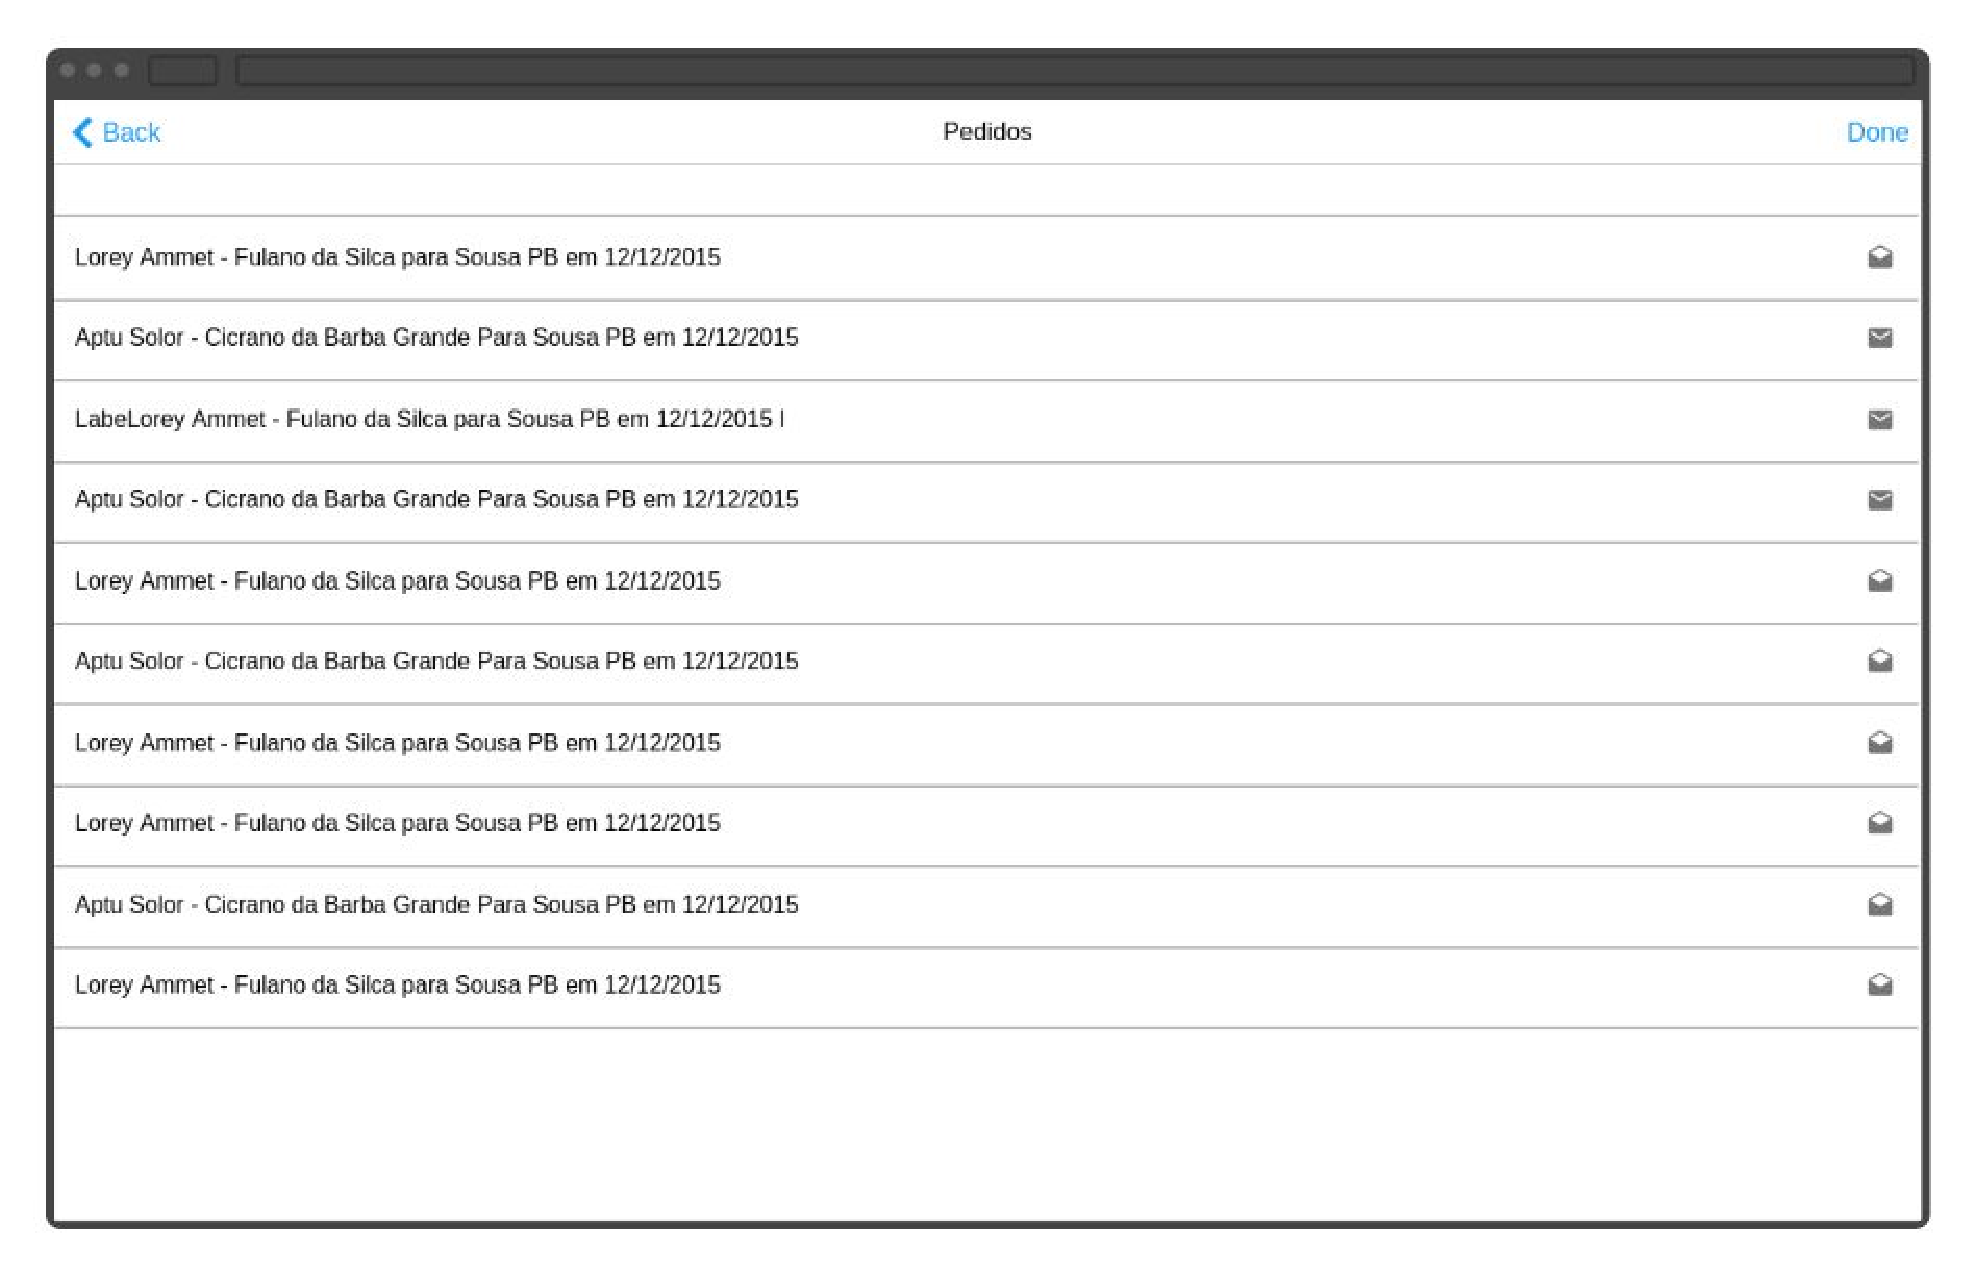
\includegraphics[width=12cm]{img/prototipos/visualizacao-pedido.eps}
% \caption{Visualização de pedidos}
% \label{figura:visualizacao_pedidos}
% \end{figure}

% \begin{figure}[H]
% \centering
% 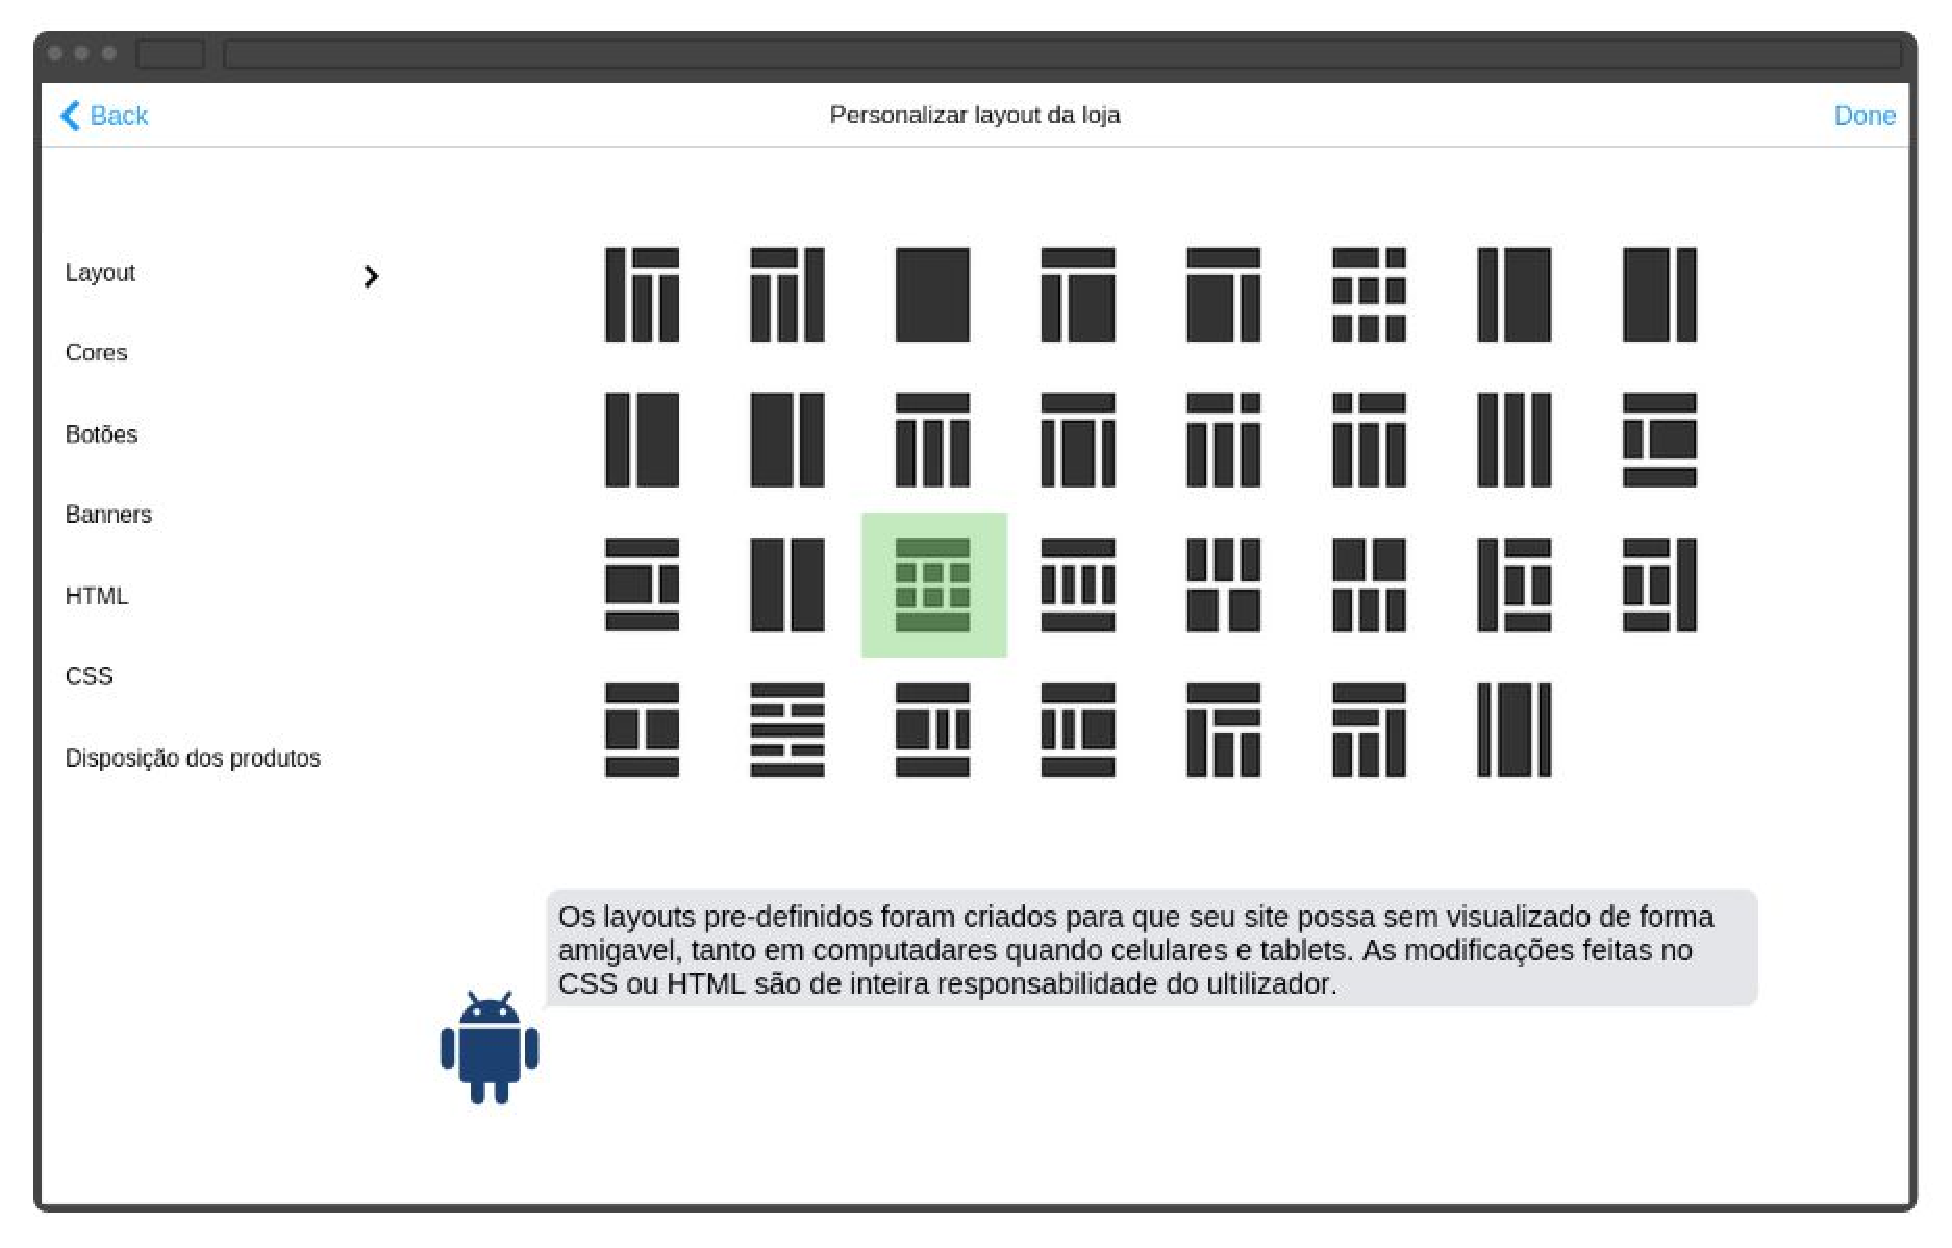
\includegraphics[width=12cm]{img/prototipos/painel-personalizacao.eps}
% \caption{Painel de Personalização}
% \label{figura:painel_personalizacao}
% \end{figure}

% \begin{figure}[H]
% \centering
% 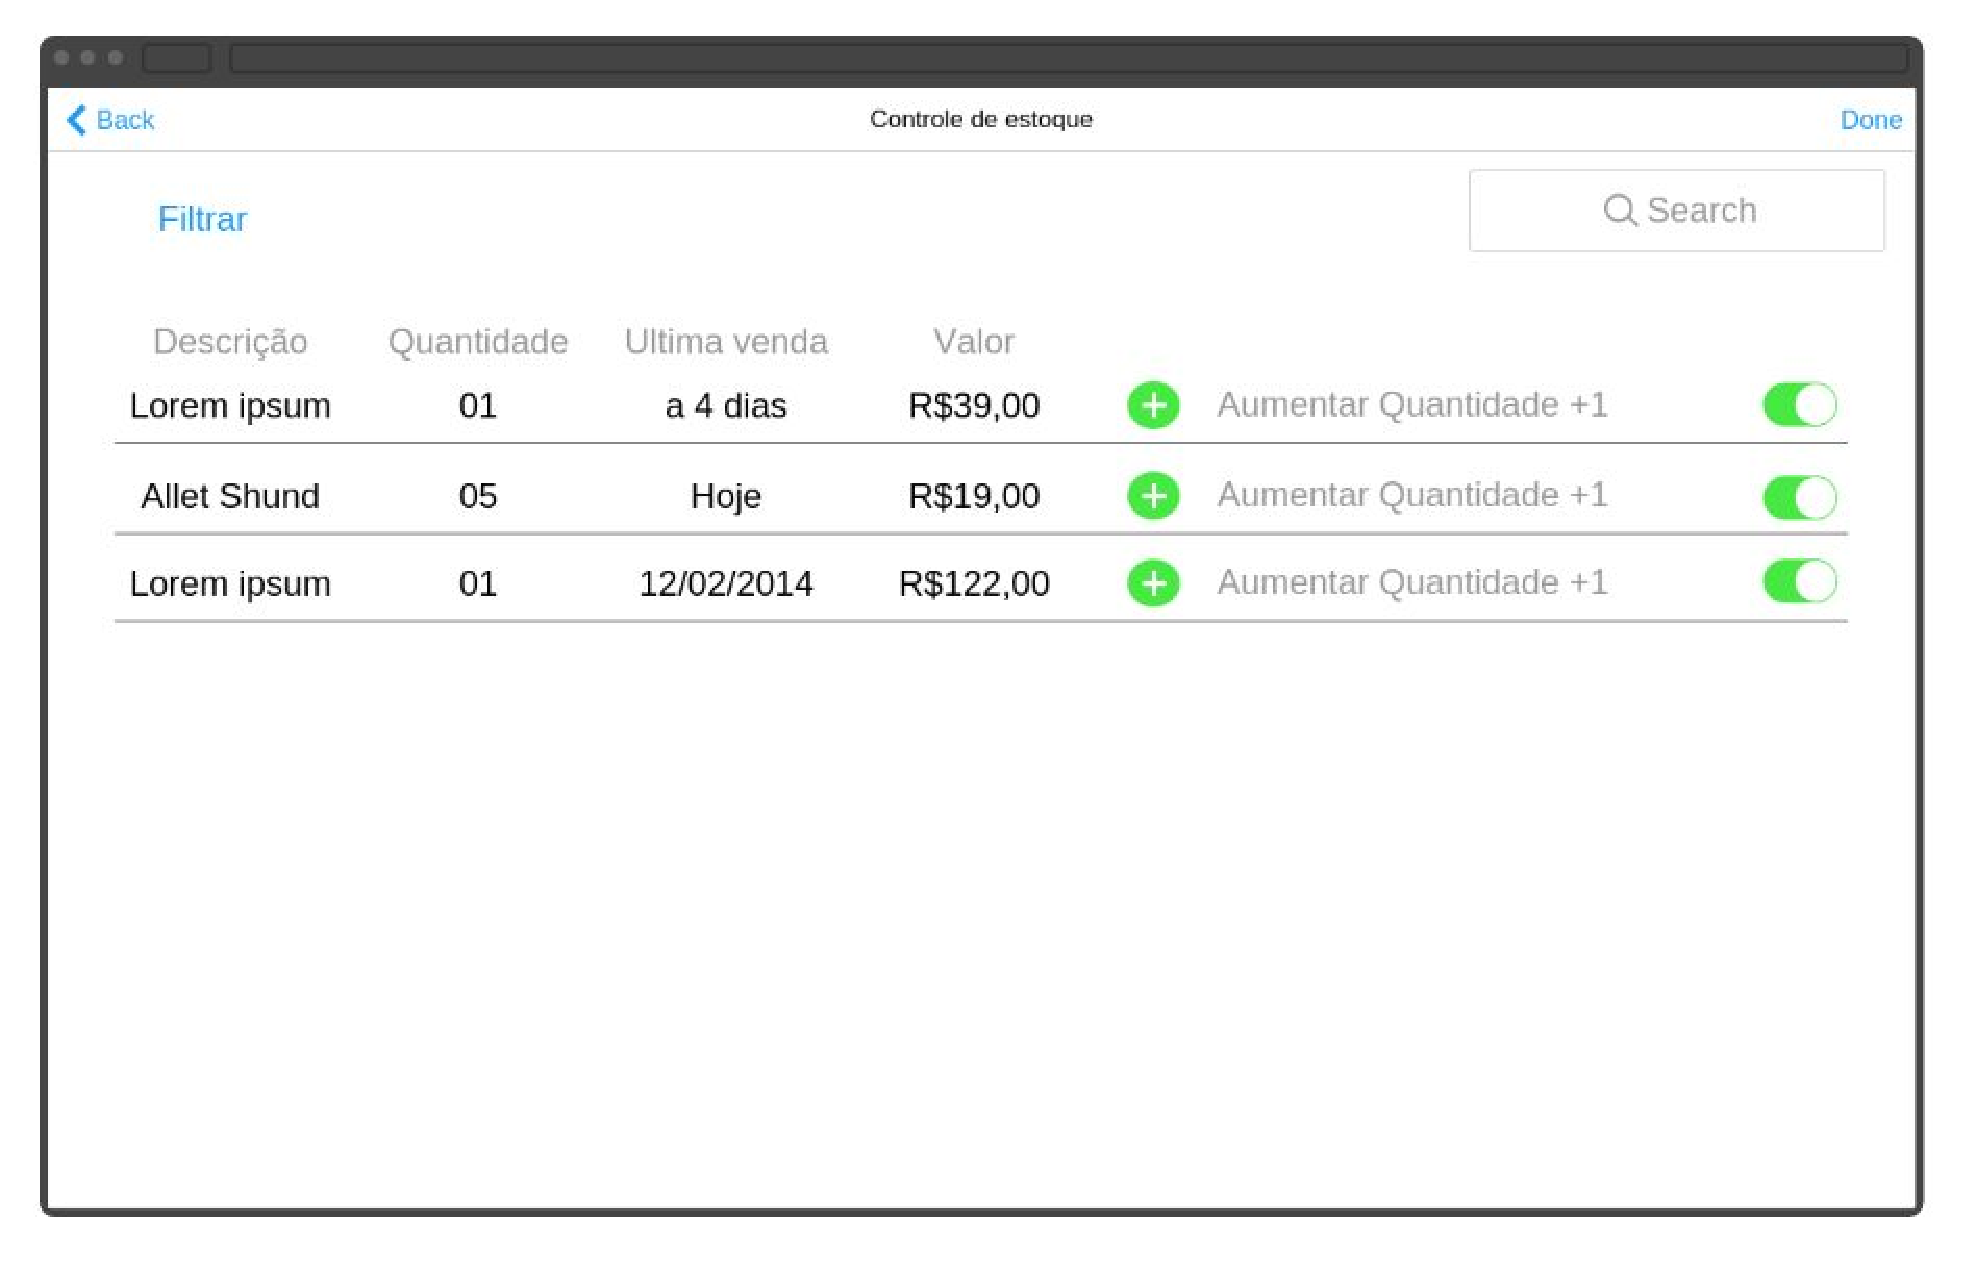
\includegraphics[width=12cm]{img/prototipos/estoque.eps}
% \caption{Controle de estoque}
% \label{figura:controle_estoque}
% \end{figure}

% \begin{figure}[H]
% \centering
% 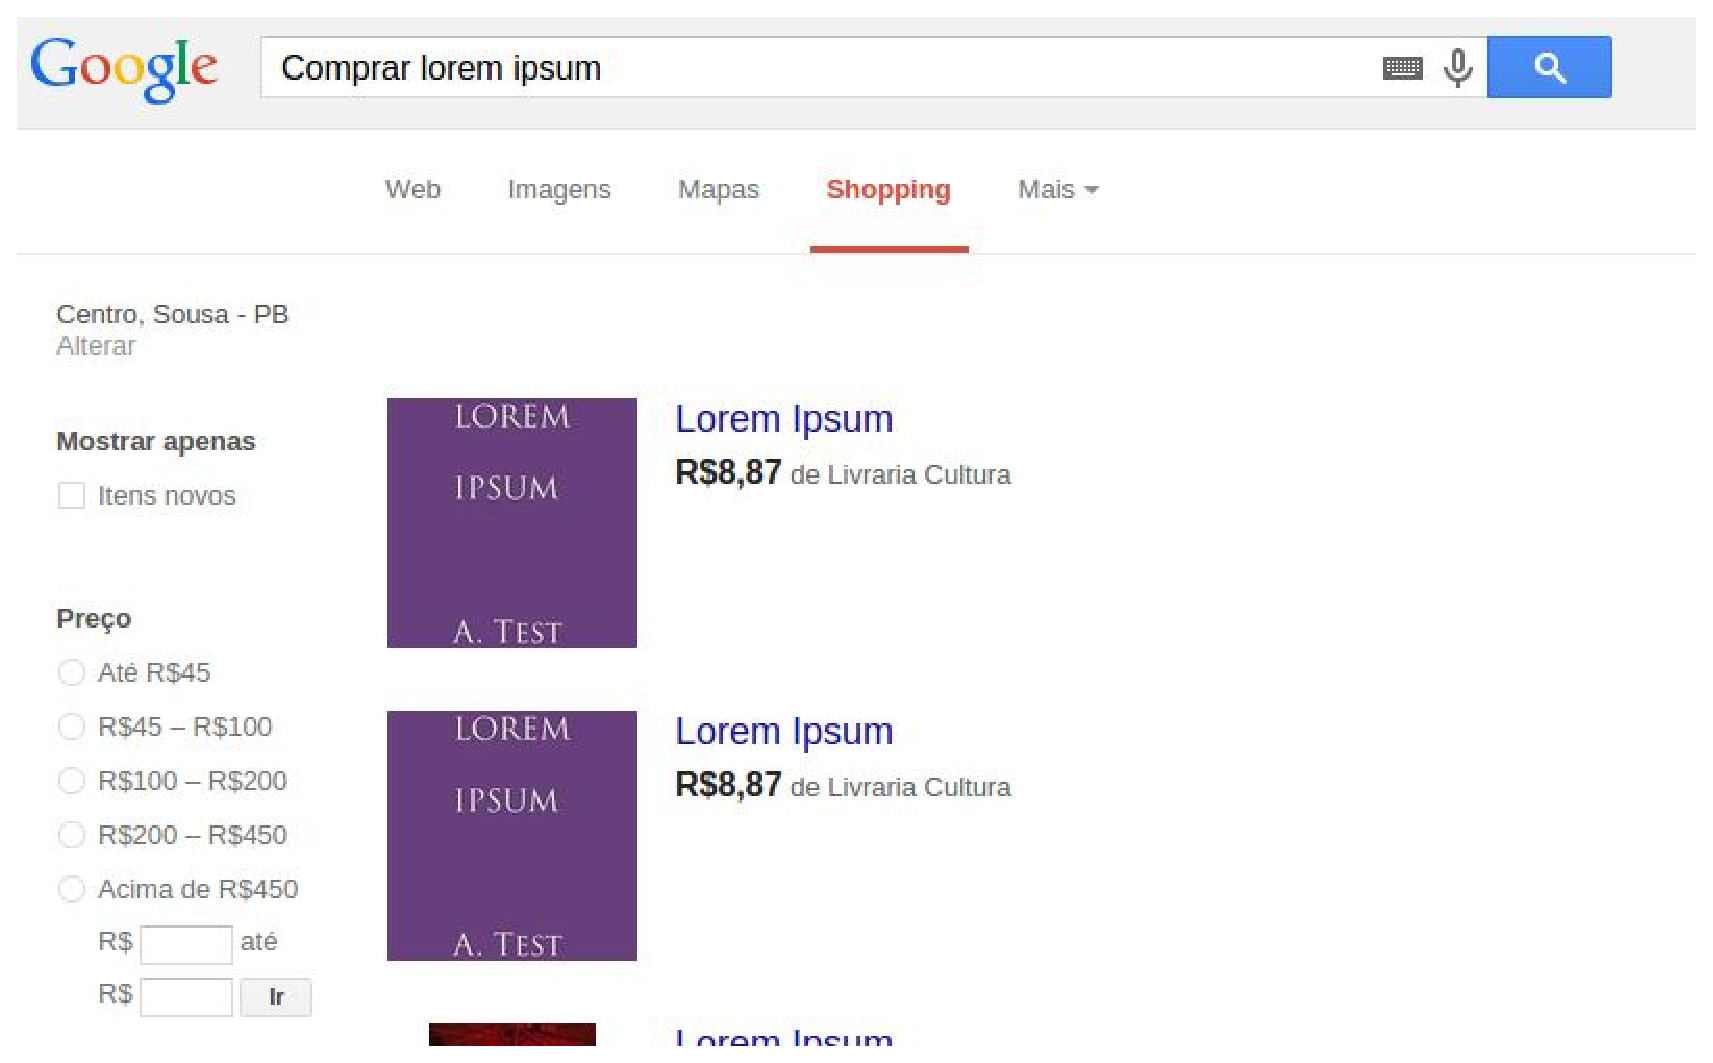
\includegraphics[width=12cm]{img/prototipos/visualizacao-gs.eps}
% \caption{Visualização dos produtos no Google Shoppinng}
% \label{figura:google_shopping}
% \end{figure}
% % section prot_tipos (end)

% \chapter{User Stories e Testes de Aceitação} % (fold)
% \label{app:user_stories_e_testes_de_aceitacao}

% \begin{longtable}{|p{1.5cm}|p{3.5cm}|c|p{2cm}|p{2cm}|c|}
% \hline
% \multicolumn{6}{|c|}{\textbf{\textit{User Story} 01}}\\
% \hline		
% \rowcolor{ballblue}
% Tarefa & Descrição & Responsável & Estimativa de tempo (horas) & Tempo real (horas) & Status\\
% \hline
% T1 & Implementar Script para salvar um Usuário Lojista & João Marcos & 2 & 1 & Finalizado\\
% \hline
% T2 & Implementar Script para validar informações do usuário Lojista & João Marcos & 2 & 1 & Finalizado\\
% \hline
% T3 & Criar Formulário para cadastro usuários lojistas & João Marcos & 3 & 2 & Finalizado\\	
% \hline
% T5 & Criar página editar as informações do usuário Lojista & João Marcos & 4 & 3 & Finalizado\\	
% \hline
% \caption{Alocação de Tarefas - US01}
% \label{quadro:tat-us03}
% \end{longtable}

% \begin{longtable}{|l|p{11.8cm}|c|}
% \hline
% \multicolumn{3}{|c|}{\textbf{\textit{User Story} 01}}\\
% \hline		
% \rowcolor{ballblue}
% \multicolumn{2}{|c|}{Testes de aceitação} & Status\\	
% \hline
% TA1 & Dado que estou na página de registro de novo usuário, quando eu preencher o formulário com os dados obrigatórios de forma correta , o usuário deve ser salvo.   & Finalizado\\
% \hline
% TA2 & Dado que estou na página de registro de novo usuário, quando eu preencher o formulário com os dados obrigatórios de forma incorreta , o usuário não deve ser salvo e uma mensagem de erro deve ser exibida.   & Finalizado\\
% \hline
% TA3 & Dado que estou acessando a ficha de edição de informações sobre o Lojista, quando eu alterar alguma informação do formulário com os dados válidos, o usuário deve ser atualizado e uma mensagem de sucesso deve ser exibida.   & Finalizado\\
% \hline
% TA4 & Dado que estou acessando a ficha de edição de informações sobre o Lojista, quando eu alterar alguma informação do formulário com os dados inválidos, tais informações não serão salvas e uma mensagem de erro deve ser exibida.   & Finalizado\\
% \hline	
% \caption{Teste de aceitação - US01}
% \label{quadro:teste-aceitacao-us01}
% \end{longtable}

% \begin{longtable}{|p{1.5cm}|p{3.5cm}|c|p{2cm}|p{2cm}|c|}
% \hline
% \multicolumn{6}{|c|}{\textbf{\textit{User Story} 02}}\\
% \hline		
% \rowcolor{ballblue}
% Tarefa & Descrição & Responsável & Estimativa de tempo (horas) & Tempo real (horas) & Status\\
% \hline
% T1 & Implementar Script para salvar uma Loja & João Marcos & 2 & 1 & Finalizado\\
% \hline
% T2 & Implementar Script para validar informações do de uma Loja & João Marcos & 2 & 1 & Finalizado\\
% \hline
% T3 & Criar Formulário para cadastro de uma Loja & João Marcos & 3 & 2 & Finalizado\\	
% \hline
% T5 & Criar página editar as informações Sobre uma Loja & João Marcos & 4 & 3 & Finalizado\\
% \hline
% \caption{Alocação de Tarefas - US01}
% \label{quadro:tat-us03}
% \end{longtable}

% \begin{longtable}{|l|p{11.8cm}|c|}
% \hline
% \multicolumn{3}{|c|}{\textbf{\textit{User Story} 02}}\\
% \hline		
% \rowcolor{ballblue}
% \multicolumn{2}{|c|}{Testes de aceitação} & Status\\	
% \hline
% TA1 & Dado que estou na página de criação de uma Loja, quando eu preencher o formulário com os dados obrigatórios de forma correta , a loja ser salva.   & Finalizado\\
% \hline
% TA2 & Dado que estou na página criação de uma Loja, quando eu preencher o formulário com os dados obrigatórios de forma incorreta , a Loja não deve ser salva e uma mensagem de erro deve ser exibida.   & Finalizado\\
% \hline
% TA3 & Dado que estou acessando a página de edição de informações sobre uma Loja, quando eu alterar alguma informação do formulário com os dados válidos, a Loja deve ser atualizada e uma mensagem de sucesso deve ser exibida.   & Finalizado\\
% \hline
% TA4 & Dado que estou acessando a página de edição de informações sobre uma Loja, quando eu alterar alguma informação do formulário com os dados inválidos, tais informações não serão salvas e uma mensagem de erro deve ser exibida.   & Finalizado\\
% \hline	
% TA5 & Permitir que eu possa cadastrar mais de uma Loja no sistema.  & Finalizado\\
% \hline	
% \caption{Teste de aceitação - US02}
% \label{quadro:teste-aceitacao-us02}
% \end{longtable}

% \begin{longtable}{|p{1.5cm}|p{3.5cm}|c|p{2cm}|p{2cm}|c|}
% \hline
% \multicolumn{6}{|c|}{\textbf{\textit{User Story} 03}}\\
% \hline		
% \rowcolor{ballblue}
% Tarefa & Descrição & Responsável & Estimativa de tempo (horas) & Tempo real (horas) & Status\\
% \hline
% T1 & Implementar Script para salvar um Produto & João Marcos & 2 & 1 & Finalizado\\
% \hline
% T2 & Implementar Script para validar informações do produto & João Marcos & 2 & 1 & Finalizado\\
% \hline
% T3 & Criar Formulário para cadastro de produto & João Marcos & 3 & 2 & Finalizado\\
% \hline
% T4 & Criar formulário para edição de produto & João Marcos & 2 & 1 & Finalizado\\
% \hline
% T5 & Criar página para o estoque, exibindo as informações básicas de cada produto com sua respectiva quantidade e link para ficha do produto & João Marcos & 4 & 3 & Finalizado\\
% \hline
% T6 & Criar botão para exclusão de um produto na página de estoque & João Marcos & 2 & 1 & Finalizado\\
% \hline
% \caption{Alocação de Tarefas - US03}
% \label{quadro:tat-us03}
% \end{longtable}

% \begin{longtable}{|l|p{11.8cm}|c|}
% \hline
% \multicolumn{3}{|c|}{\textbf{\textit{User Story} 03}}\\
% \hline		
% \rowcolor{ballblue}
% \multicolumn{2}{|c|}{Testes de aceitação} & Status\\	
% \hline
% TA1 & Dado que estou na página de cadastro de produto, quando eu preencher o formulário com os dados obrigatórios de forma correta , o produto deve ser salvo e informado uma mensagem de sucesso.   & Finalizado\\
% \hline
% TA2 & Dado que estou na página de cadastro de produto, quando eu preencher o formulário com os dados obrigatórios de forma incorreta , o produto não deve ser salvo e uma mensagem de erro deve ser exibida.   & Finalizado\\
% \hline
% TA3 & Dado que estou acessando a ficha de edição de produto, quando eu alterar alguma informação do formulário com os dados válidos, o produto deve ser atualizado e uma mensagem de sucesso deve ser exibida.   & Finalizado\\
% \hline
% TA4 & Dado que estou acessando a ficha de edição de produto, quando eu alterar alguma informação do formulário com os dados inválidos, tais informações não serão salvas e uma mensagem de erro deve ser exibida.   & Finalizado\\
% \hline
% TA5 & Dado que estou na página de estoque, quando eu selecionar a opção excluir este produto, um diálogo de confirmação deve ser exibido. Caso confirme o produto deve ser excluído  & Finalizado\\
% \hline
% TA6 & Dado que estou na página de estoque, quando eu selecionar a opção excluir este produto, um diálogo de confirmação deve ser exibido. Caso não confirme o produto não deve ser excluído  & Finalizado\\
% \hline
% \caption{Teste de aceitação - US03}
% \label{quadro:teste-aceitacao-us03}
% \end{longtable}

% \begin{longtable}{|p{1.5cm}|p{3.5cm}|c|p{2cm}|p{2cm}|c|}
% \hline
% \multicolumn{6}{|c|}{\textbf{\textit{User Story} 04}}\\
% \hline		
% \rowcolor{ballblue}
% Tarefa & Descrição & Responsável & Estimativa de tempo (horas) & Tempo real (horas) & Status\\
% \hline
% T1 & Implementar Script para validar credenciais de um lojista & João Marcos & 2 & 1 & Finalizado\\
% \hline
% T2 & Criar página inicial contendo um menu de navegação onde o usuário poderá navegar com facilidade no sistema & João Marcos & 4 & 3 & Finalizado\\
% \hline
% T3 & Criar botão para sair do Sistema & João Marcos & 2 & 1 & Finalizado\\
% \hline
% T4 & Criar página de seleção de lojas, onde o usuário poderá escolher a loja que deseja gerenciar no momento & João Marcos & 5 & 4 & Finalizado\\
% \hline
% T5 & Criar página de gerenciamento específica para lojas, que será exibida ao selecionar uma Loja na T4 & João Marcos & 4 & 2 & Finalizado\\
% \hline
% T6 & Criar menu lateral na página de gerenciamento da loja, permitindo a navegação dentre as funcionalidades inerentes ao gerenciamento da loja & João Marcos & 2 & 1 & Finalizado\\
% \hline
% \caption{Alocação de Tarefas - US04}
% \label{quadro:tat-us04}
% \end{longtable}

% \begin{longtable}{|l|p{11.8cm}|c|}
% \hline
% \multicolumn{3}{|c|}{\textbf{\textit{User Story} 04}}\\
% \hline		
% \rowcolor{ballblue}
% \multicolumn{2}{|c|}{Testes de aceitação} & Status\\	
% \hline
% TA1 & Dado que estou na página de login, quando eu preencher o formulário com os dados obrigatórios de forma correta , ser redirecionado para a página inicial do sistema.   & Finalizado\\
% \hline
% TA2 & Dado que estou na página de login, quando eu preencher o formulário com os dados obrigatórios de forma incorreta , não posso ser redirecionado para o sistema e uma mensagem de erro deve ser exibida.   & Finalizado\\
% \hline
% TA3 & Dado que estou logado, quando clicar no botão sair, devo ser desconectado do sistema, onde terei que fazer login novamente caso queira entrar no sistema novamente.   & Finalizado\\
% \hline
% TA4 & Dado que estou na página de seleção de lojas, quando selecionar uma loja, devo ser redirecionado  para página inicial de gerenciamento da Loja selecionada.  & Finalizado\\
% \hline
% TA5 & Dado que estou logado, quando eu selecionar uma opção do menu lateral, devo ser redirecionado para página especificada  & Finalizado\\
% \hline	
% \caption{Teste de aceitação - US04}
% \label{quadro:teste-aceitacao-us04}
% \end{longtable}

% chapter user_stories_e_testes_de_aceita_o (end)

\end{document}
